\ifdefined\handoutmode
  \PassOptionsToClass{handout}{beamer}
\fi
\documentclass[aspectratio=169]{beamer}

\input{../../../../hh_bpa_forel-preamble} % this is ugly.

\title{FMTS mätteknik HT2026 -- Dag 2}
\author{Pererik Andreasson \\ Struan Gray }
\date{\today{}}

\begin{document}

%%% Title slide: different footer, large logo
{
% no page #, no logo on title page
\setbeamertemplate{footline}{}
\setbeamertemplate{logo}{\titlelogos}
\begin{frame}
\vfill
  \begin{block}
    \maketitle
  \end{block}
\end{frame}
}

\mode<beamer>{
\frame{
    \frametitle{Lärandemål}
    {\Huge
    \begin{enumerate}
        \item<1-> Ensam mätning inget värt.
        \item<2-> Okalibrerat mätinstrument inget värt.
        \item<3-> Elektriska mätningar \emph{påverkar} mätobjektet $\rightarrow$ behöver \emph{tolkas}.
    \end{enumerate}
    }
}
} % end mode


\begin{frame}    
  \frametitle{Dagens plan}
    {\Large
        \begin{itemize}
            \item Repetera Ohms lag, mäta ström och spänning
            \item Öva spänningsdelning och kontrollmäte
            \item Närma oss gränsen för multimetern
            \item Kondensatorer i kretsar
            \item AC - växelström
            \item RMS vs. True RMS
        \end{itemize}
    }
\end{frame}   


\mode<beamer>{
\frame{
    \frametitle{}
    {\Huge Multimetermätningar och Ohms lag}
} % end frame


\frame{
    \frametitle{}
    \begin{tikzpicture}[remember picture,overlay]
        \node[at=(current page.center)] {
            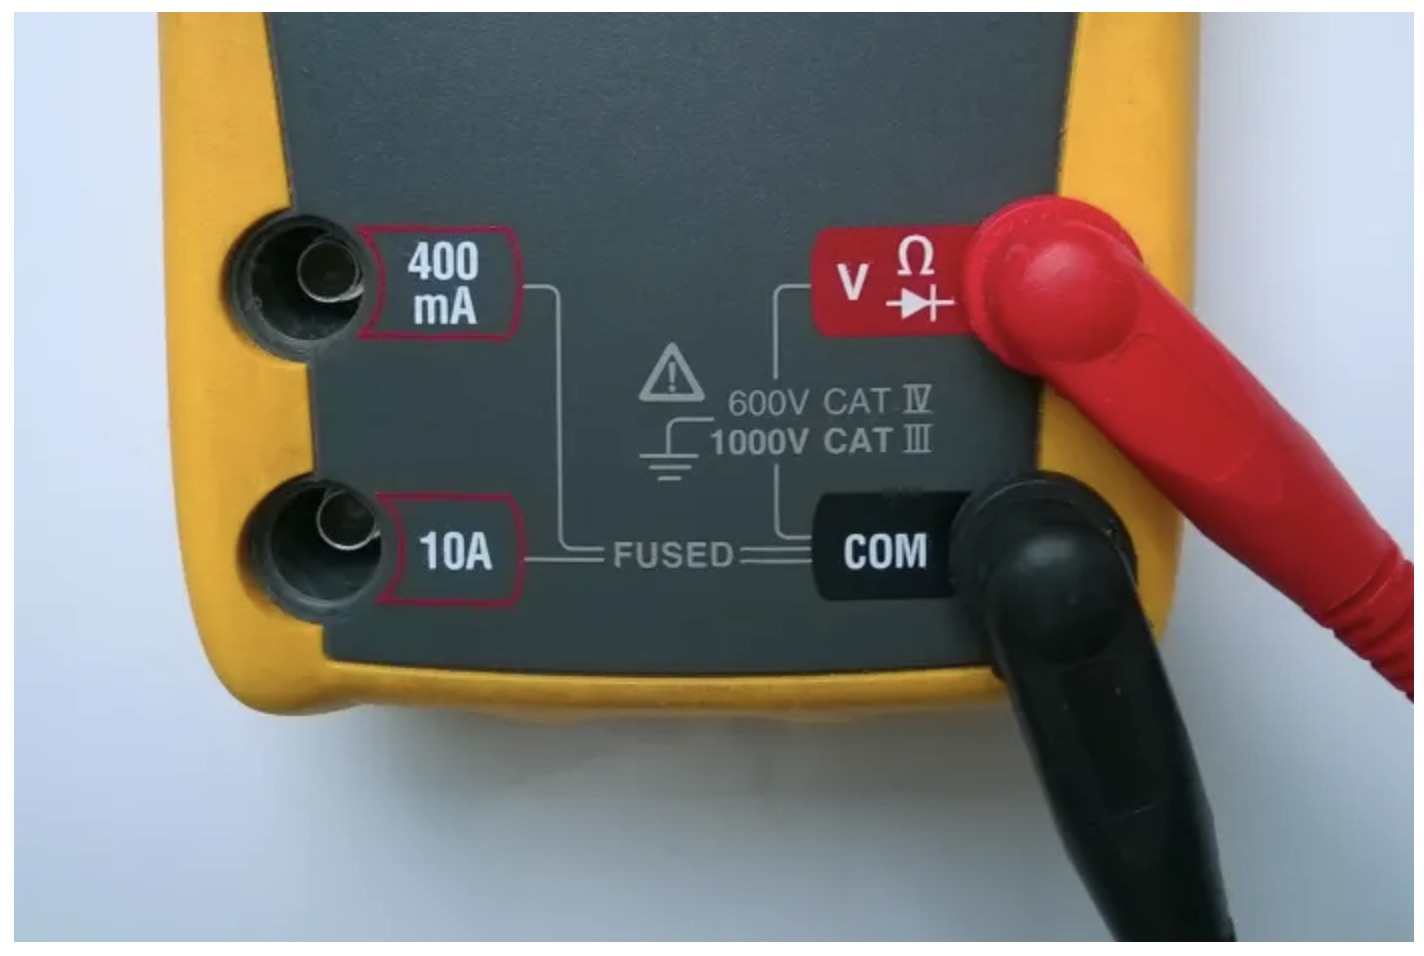
\includegraphics[keepaspectratio,
                                 width=\paperwidth,
                                 height=\paperheight]{figures/multimeter_probes_voltage.png}
            };
   			% Varför skall vi lära oss detta?
			\onslide<1->{
			\node[rotate=30, white] at (6,2){{\Huge Ganska säkert!}};
			}
    \end{tikzpicture}    
    }


\frame{
    \frametitle{}
    \begin{tikzpicture}[remember picture,overlay]
        \node[at=(current page.center)] {
            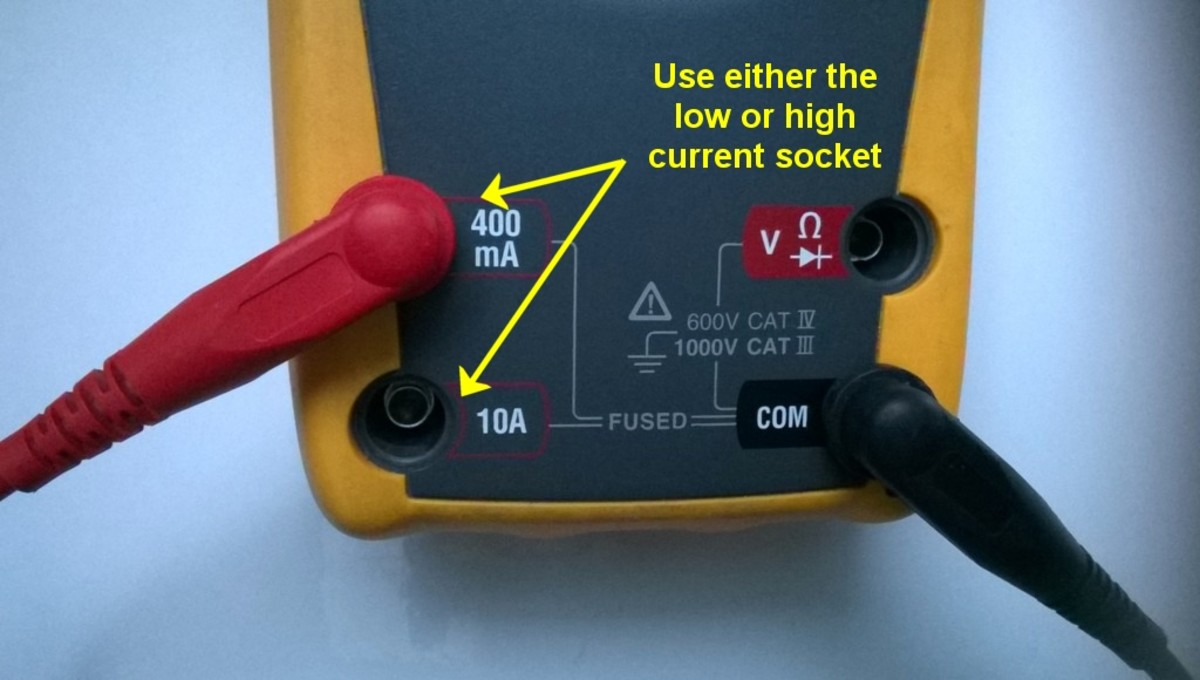
\includegraphics[keepaspectratio,
                                 width=\paperwidth,
                                 height=\paperheight]{figures/multimeter_probes_current.jpg}
            };
   			% Varför skall vi lära oss detta?
			\onslide<1->{
			\node[rotate=30, white] at (3,0.5){{\Huge  Osäkert! Varning!}};
			}
    \end{tikzpicture}    
    }
} % end mode


\frame{
\frametitle{Mäta spänning}
\resizebox{\textwidth}{!}{%
\begin{minipage}{.5\textwidth}
\centering
\begin{tikzpicture}[scale = 1, american]
    \draw (0, 0) 
    node[ground, rotate=-90] {}
    to[american voltage source=\qty{5}{\V}, invert, *-] (0, 2) 
    -- (2, 2) 
    to[R=\qty{470}{\ohm}, i=$I$] (2, 0)
	-- (0, 0)
    ;
    \draw (2, 2) 
    to[short,*-] (4, 2) 
    to[voltmeter] (4, 0) 
    to[short, -*] (2, 0) 
    ;
\end{tikzpicture}\\
Spänning \alert{över} komponenter!
\end{minipage}}
}


\handoutnoteslide


\frame{
\frametitle{Mäta ström}
\resizebox{\textwidth}{!}{%
\begin{minipage}{.5\textwidth}
\centering
\begin{tikzpicture}[scale = 1, american]
    \draw (0, 0) 
    node[ground, rotate=-90] {}
    to[american voltage source=\qty{5}{\V}, invert, *-] (0, 2) 
    to[short, -*] (0.5, 2)
    to[ammeter,-*] (2.5, 2) 
    -- (3, 2)
    to[R=\qty{470}{\ohm}, i=$I$] (3, 0)
	-- (0, 0)
    ;
%    \draw (2, 2) 
%    to[short,*-] (4, 2) 
%    to[ammeter] (4, 0) 
%    to[short, -*] (2, 0)
%    ;
\end{tikzpicture}\\
Ström \alert{genom} komponenter!
\end{minipage}}
}


\handoutnoteslide


\frame{
\frametitle{Mäta motstånd}
\resizebox{\textwidth}{!}{%
\begin{minipage}{.5\textwidth}
\centering
\begin{tikzpicture}[scale = 1, american]
    \draw (2, 2) 
    to[R=\qty{470}{\ohm}] (2, 0)
    ;
    \draw (2, 2) 
    to[short, -*] (3, 2)
    -- (4,2)
    to[ohmmeter] (4, 0) 
    -- (3, 0)
    to[short, *-] (2, 0)
    ;
\end{tikzpicture}\\
Koppla loss komponenter!
\end{minipage}}
}


\handoutnoteslide


\frame{
    \frametitle{}
    \begin{tikzpicture}[remember picture,overlay]
        \node[at=(current page.center)] {
            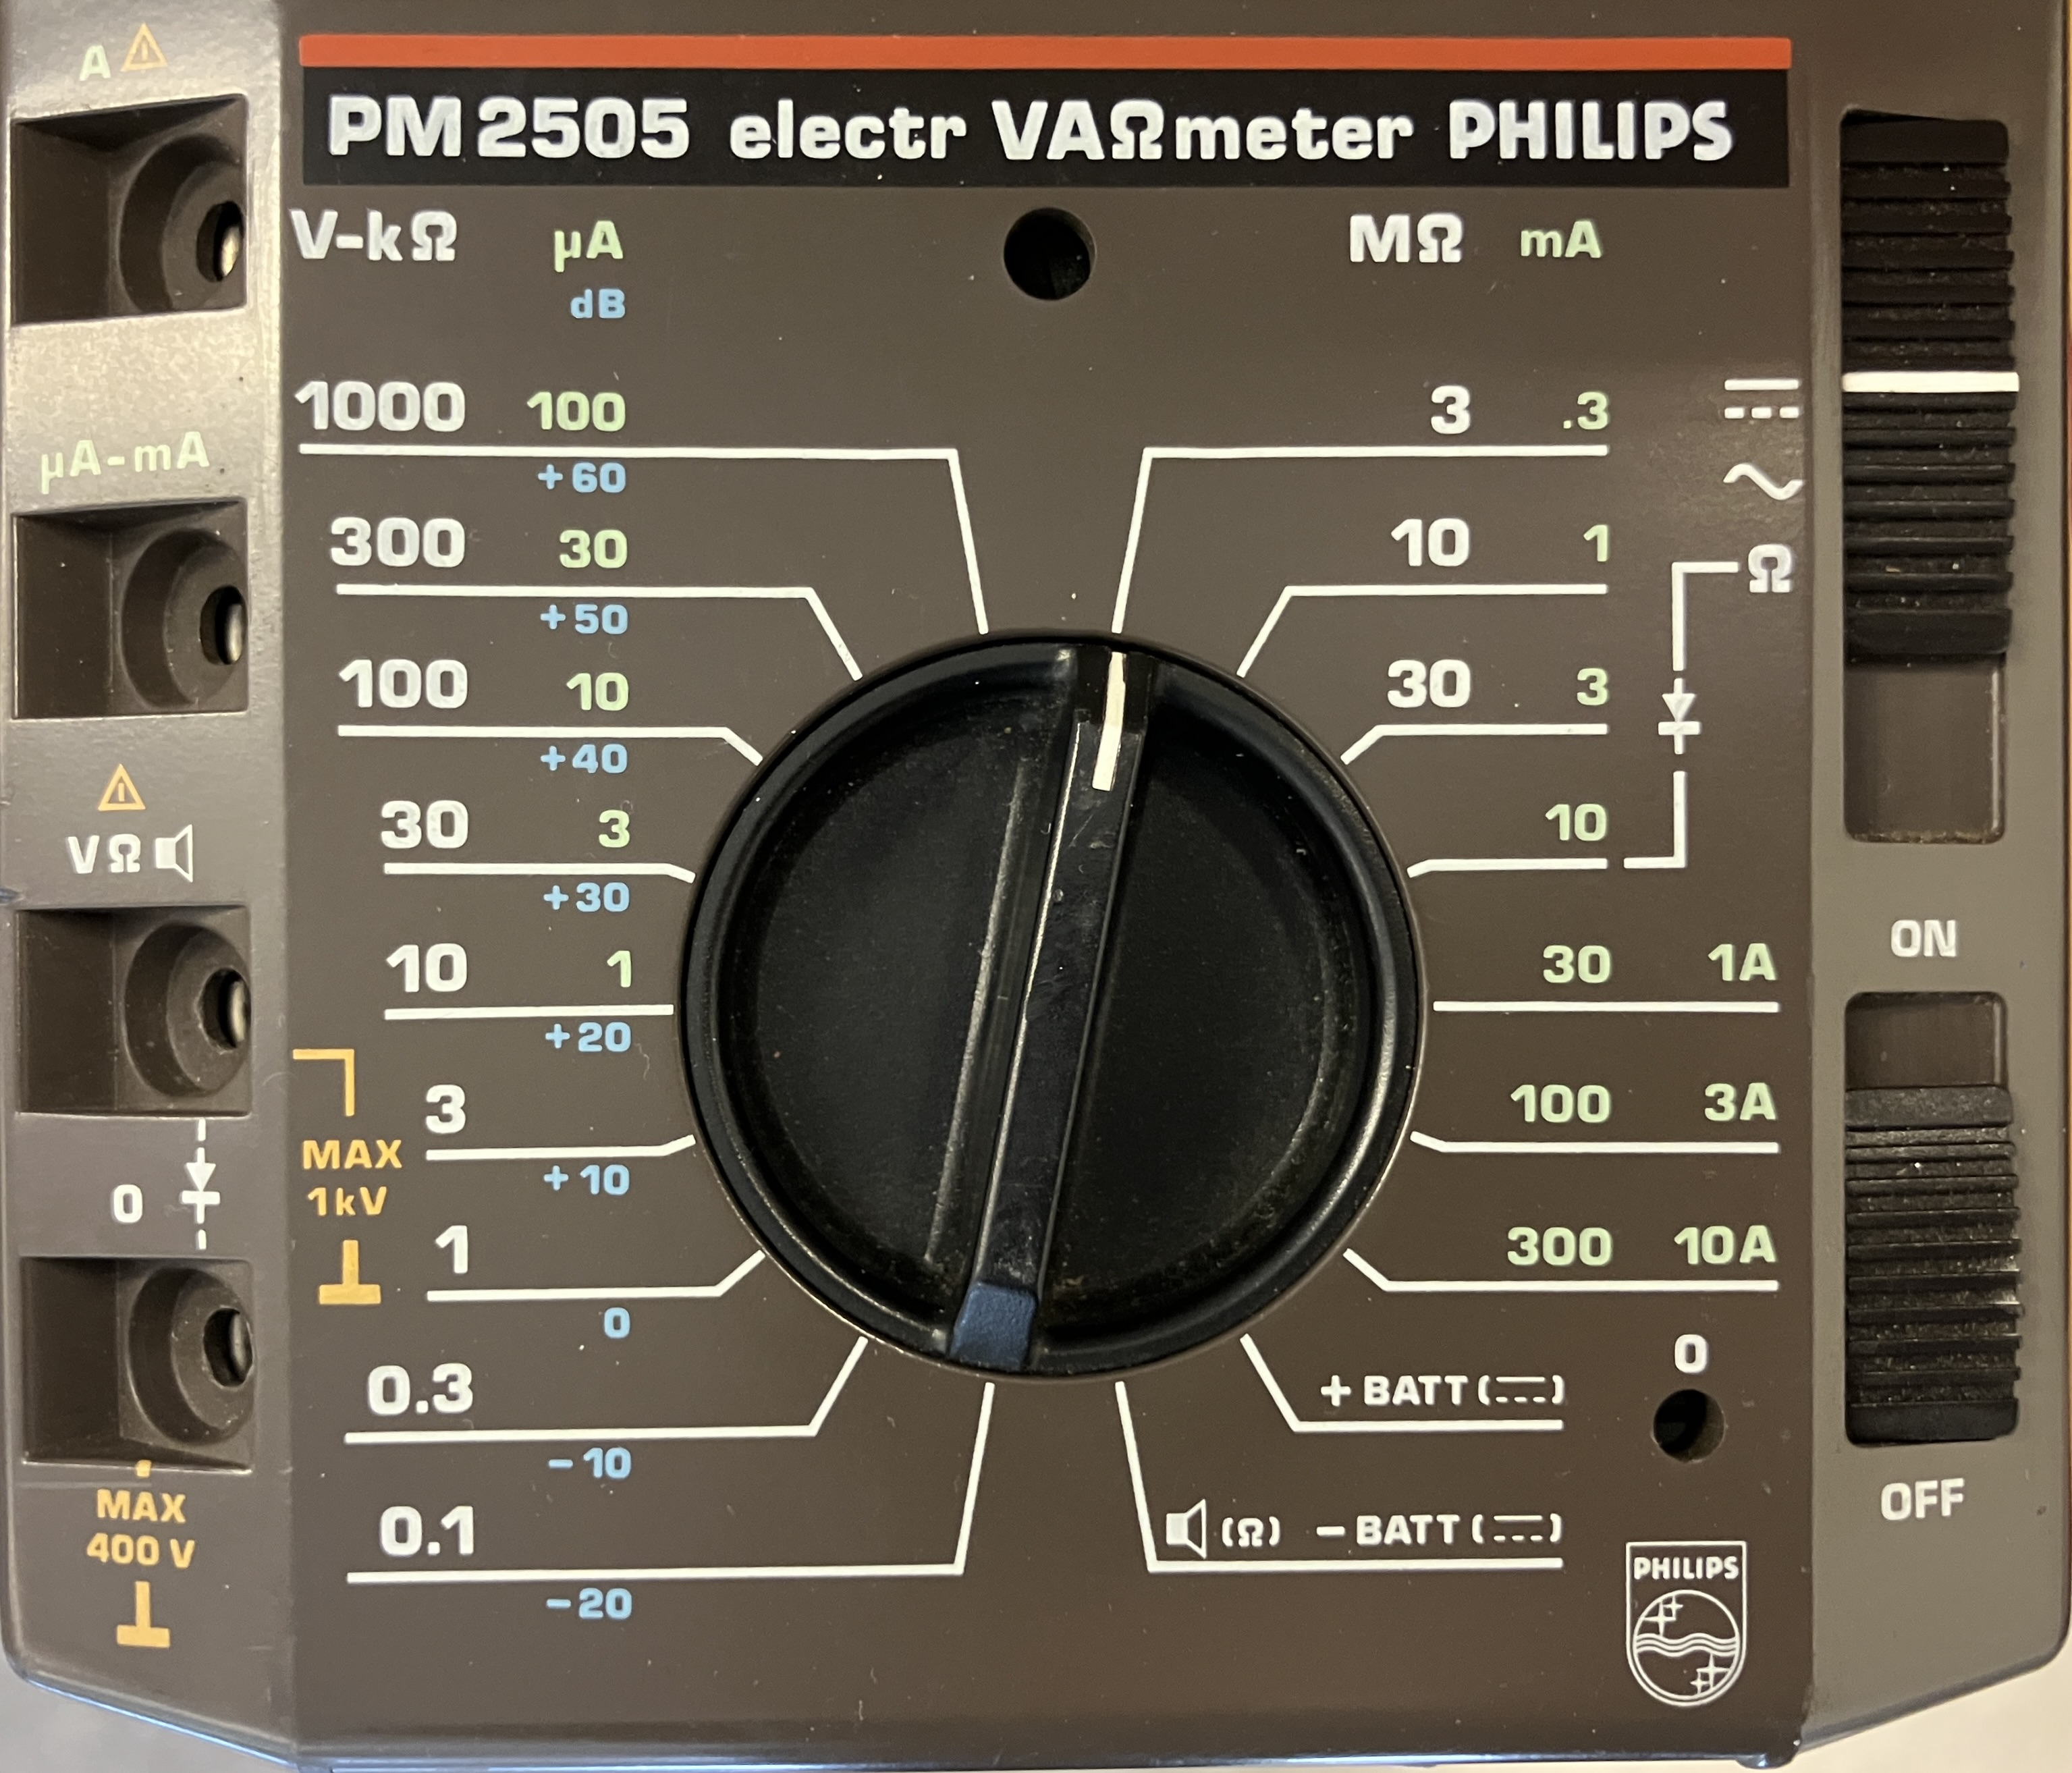
\includegraphics[keepaspectratio,
                                 width=\paperwidth,
                                 height=\paperheight]{figures/philips.JPG}
            };
   			% Varför skall vi lära oss detta?
			\onslide<1->{
			\node[rotate=0, white] at (5, 2.5){{\Huge Klurigt!}};
			}
    \end{tikzpicture}    
}


\handoutnoteslide


\frame{
\frametitle{Ohms lag-repetition}
{\Large Beräkna $I_1$ och $I_2$.}
\resizebox{0.75\textwidth}{!}{%
\begin{minipage}{.5\textwidth}
\centering
\begin{tikzpicture}[american]
    \draw (0, 0)
        to[american voltage source=\qty{50}{\V},invert] (0, 1.5)
        to[R=\qty{300}{\ohm}] (3, 1.5)
        to[short, i=$I_1$] (3, 0)
        to[R=\qty{100}{\ohm}] (0, 0)
        ;
    \draw (0.5, 1.5) 
        to[short,i=$I_2$, *-] (0.5, 3)
        to[R=\qty{200}{\ohm}] (2.5, 3)
        to[short, -*] (2.5, 1.5)
        ;
\end{tikzpicture}
\end{minipage}
}
}


\handoutnoteslide


\frame{
\frametitle{Effektbegränsning}
{\Large Två 1/4-wattsmotstånd på \qty{56}{\ohm} och \qty{39}{\ohm} kopplas i serie till en spänning $U$. Beräkna hur stor $U$ högst får vara utan att något av motstånden överbelastas.}
\resizebox{0.75\textwidth}{!}{%
\begin{minipage}{.5\textwidth}
\centering
\begin{tikzpicture}[american]
    \draw (0, 0)
        -- (0, 2)
        to[R=\qty{56}{\ohm}] (2, 2)
        to[R=\qty{39}{\ohm}] (4, 2)
        -- (4, 0)
        to[american voltage source=$U$, invert] (0, 0)
        ;
\end{tikzpicture}
\end{minipage}
}
}


\handoutnoteslide


\frame{
\frametitle{Mätrepetition}
{\Large Koppla upp kretsen nedan (krysset är en lampa). Källspänningen $U$ skall sättas till det som står på lampan (\qty{4}{\V} eller \qty{8}{\V} typiskt). Mät ström och spänning och beräkna lampans resistans.}
\resizebox{0.75\textwidth}{!}{%
\begin{minipage}{.5\textwidth}
\centering
\begin{tikzpicture}[american]
    \draw (0, 0)
        -- (0, 1.5)
        to[lamp] (2, 1.5)
        to[ammeter] (4,1.5)
        -- (4, 0)
        to[american voltage source=$U$, invert] (0, 0)
        ;
    \draw (0, 1.5) 
        to[short, *-] (0, 3) 
        to[voltmeter] (2, 3)
        to[short, -*] (2, 1.5);
\end{tikzpicture}
\end{minipage}
}
}


\handoutnoteslide


\frame{
\frametitle{Mätrepetition}
{\Large Koppla \emph{ur} lampan och mät dess resistans med Multimetern.}
\resizebox{0.75\textwidth}{!}{%
\begin{minipage}{.5\textwidth}
\centering
\begin{tikzpicture}[american]
    \draw (0, 1.5)
        to[lamp] (2, 1.5)
        ;
    \draw (0, 1.5) 
        to[short, -*] (0, 2.25) 
        -- (0, 3)
        to[ohmmeter] (2, 3)
        to[short, -*] (2, 2.25)
        -- (2, 1.5)
        ;
\end{tikzpicture}\\\vspace{5mm}
\onslide<2->{Skall vara ungefär samma?}
\end{minipage}
}
}

\handoutnoteslide

\mode<beamer>{
%%--------------------------------------------------
%% Ny frame - fullscreen bild
%%--------------------------------------------------
{ % all template changes are local to this group.
  \setbeamertemplate{navigation symbols}{}
  \begin{frame}<article:0>[plain]
    \begin{tikzpicture}[remember picture,overlay]
      \node[at=(current page.center)] {
        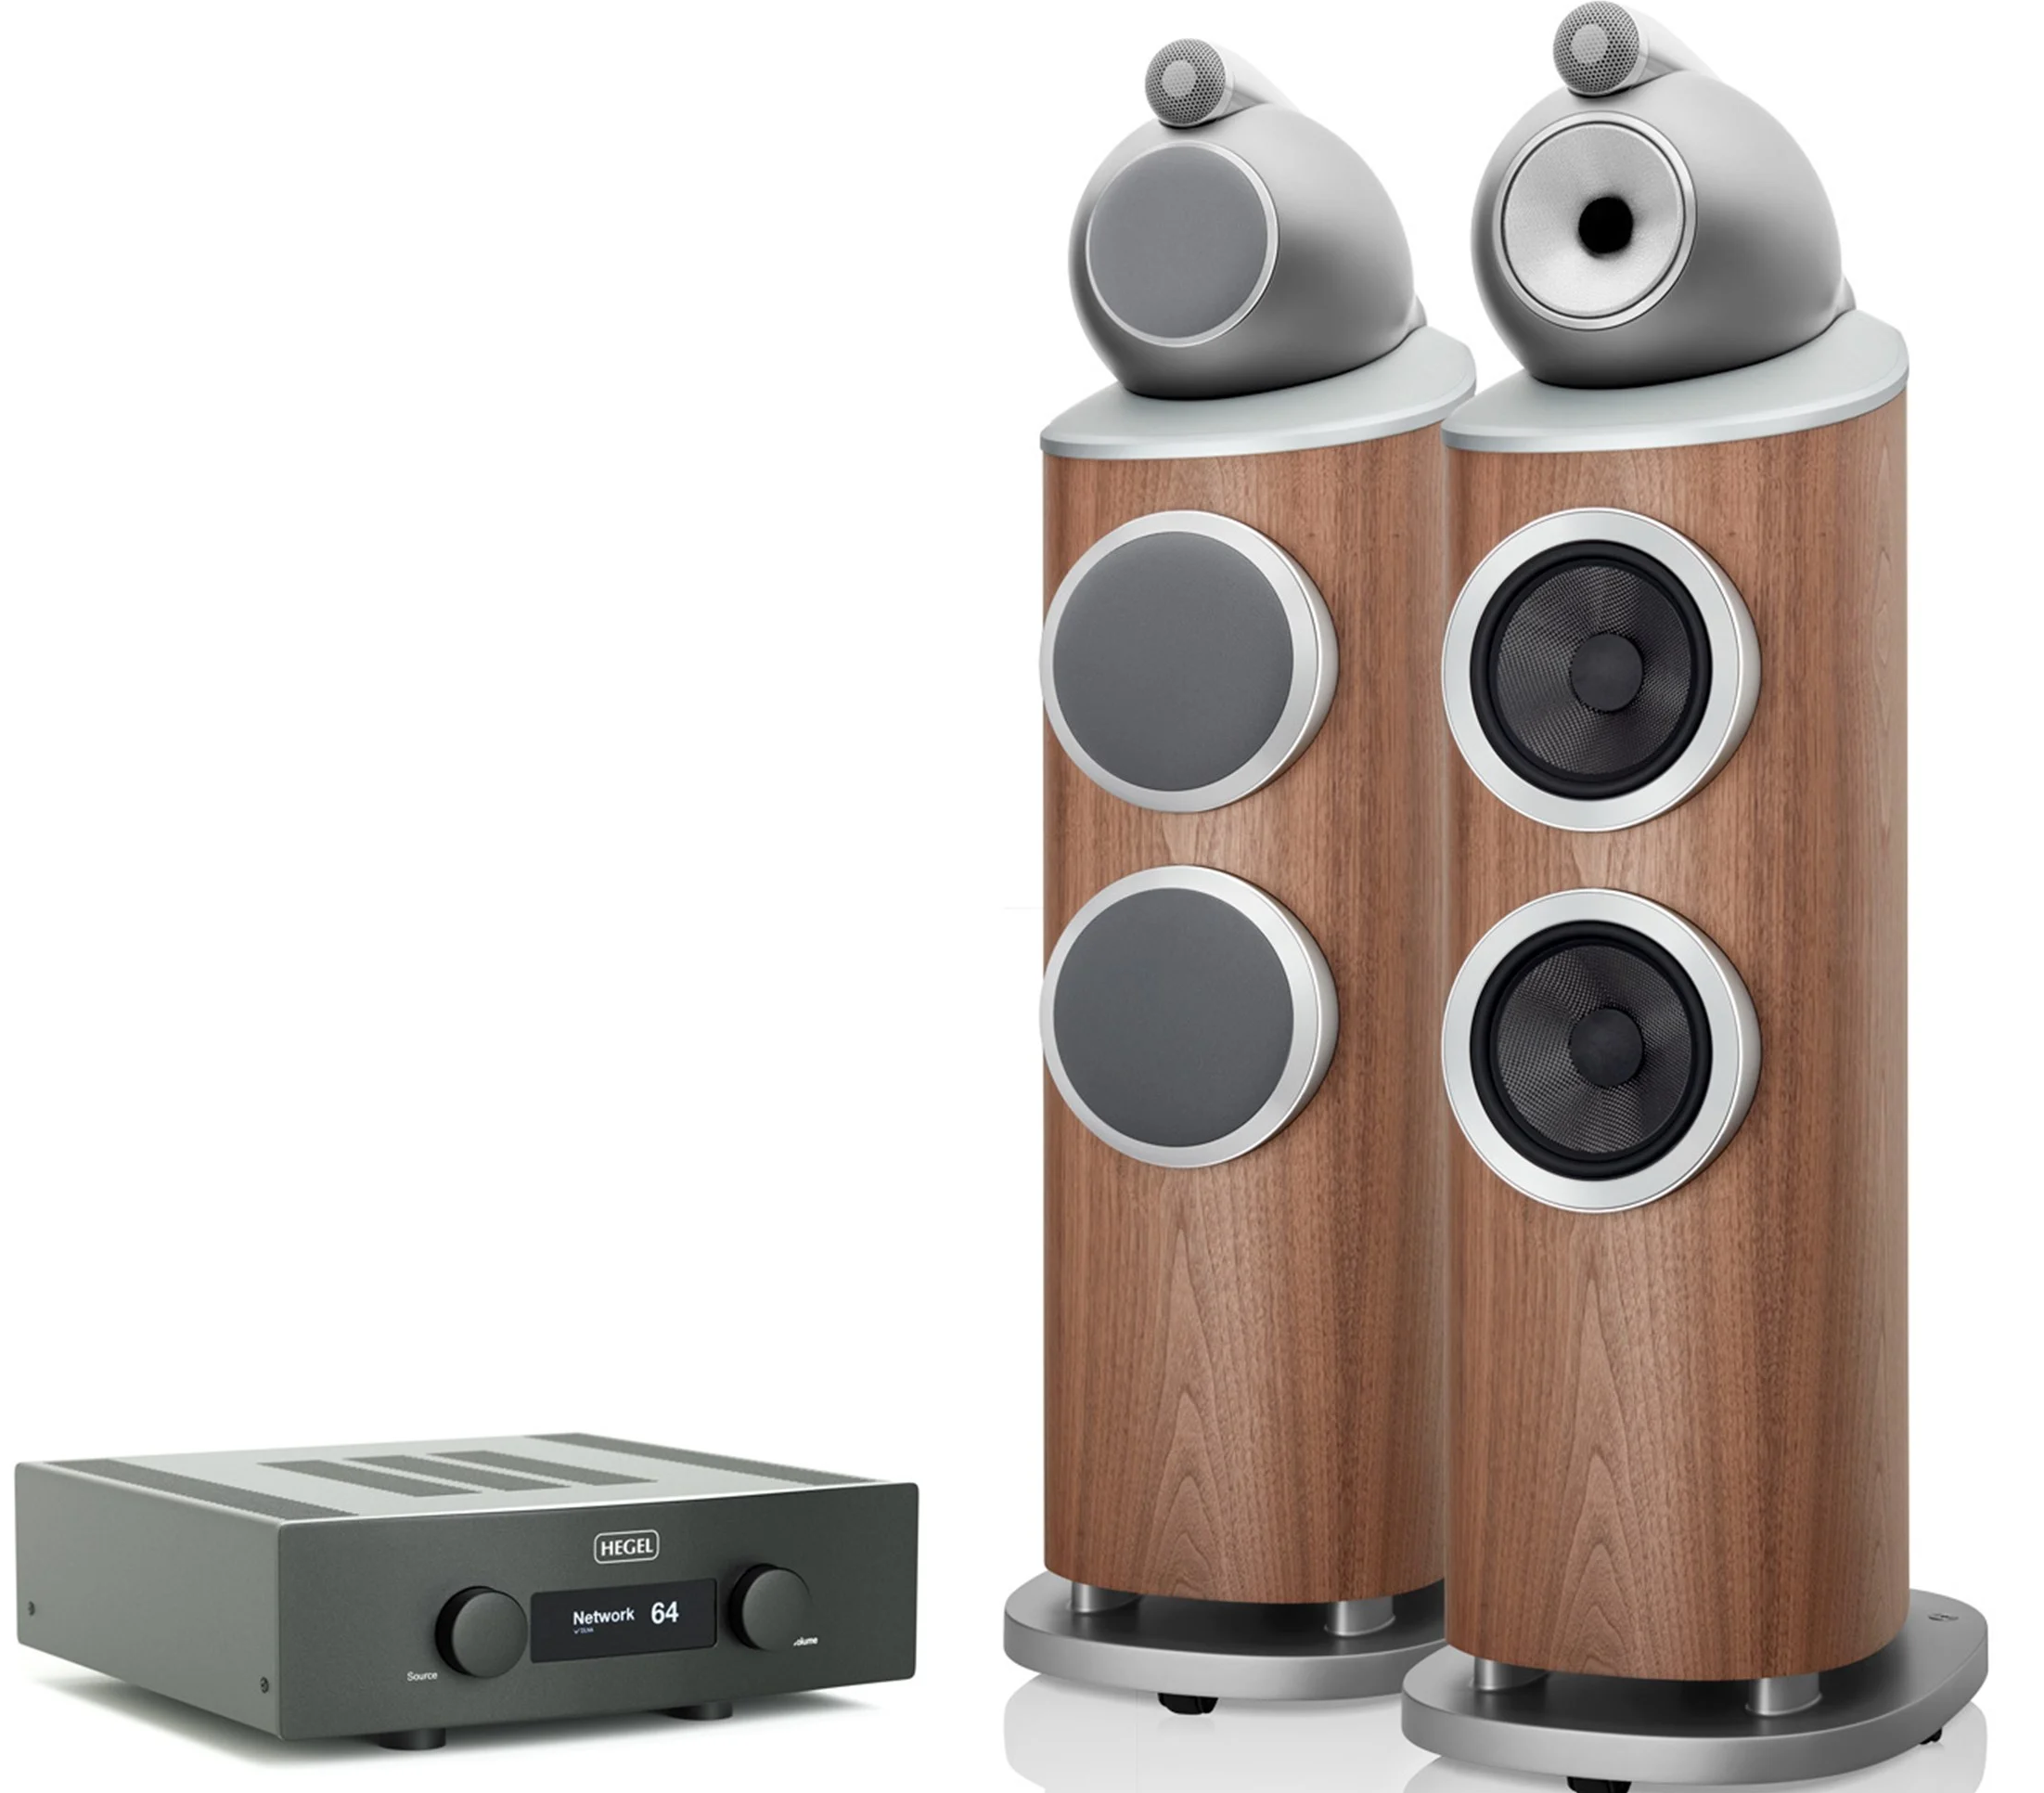
\includegraphics[keepaspectratio,
        width=\paperwidth,
        height=\paperheight]{figures/effektanpassning01.png}
      };
    \end{tikzpicture}
  \end{frame}
}
} % end mode

%%--------------------------------------------------
%% Ny frame - fullscreen bild
%%--------------------------------------------------
{ % all template changes are local to this group.
  \setbeamertemplate{navigation symbols}{}
  \begin{frame}<article:0>[plain]
    \begin{tikzpicture}[remember picture,overlay]
      \node[at=(current page.center)] {
        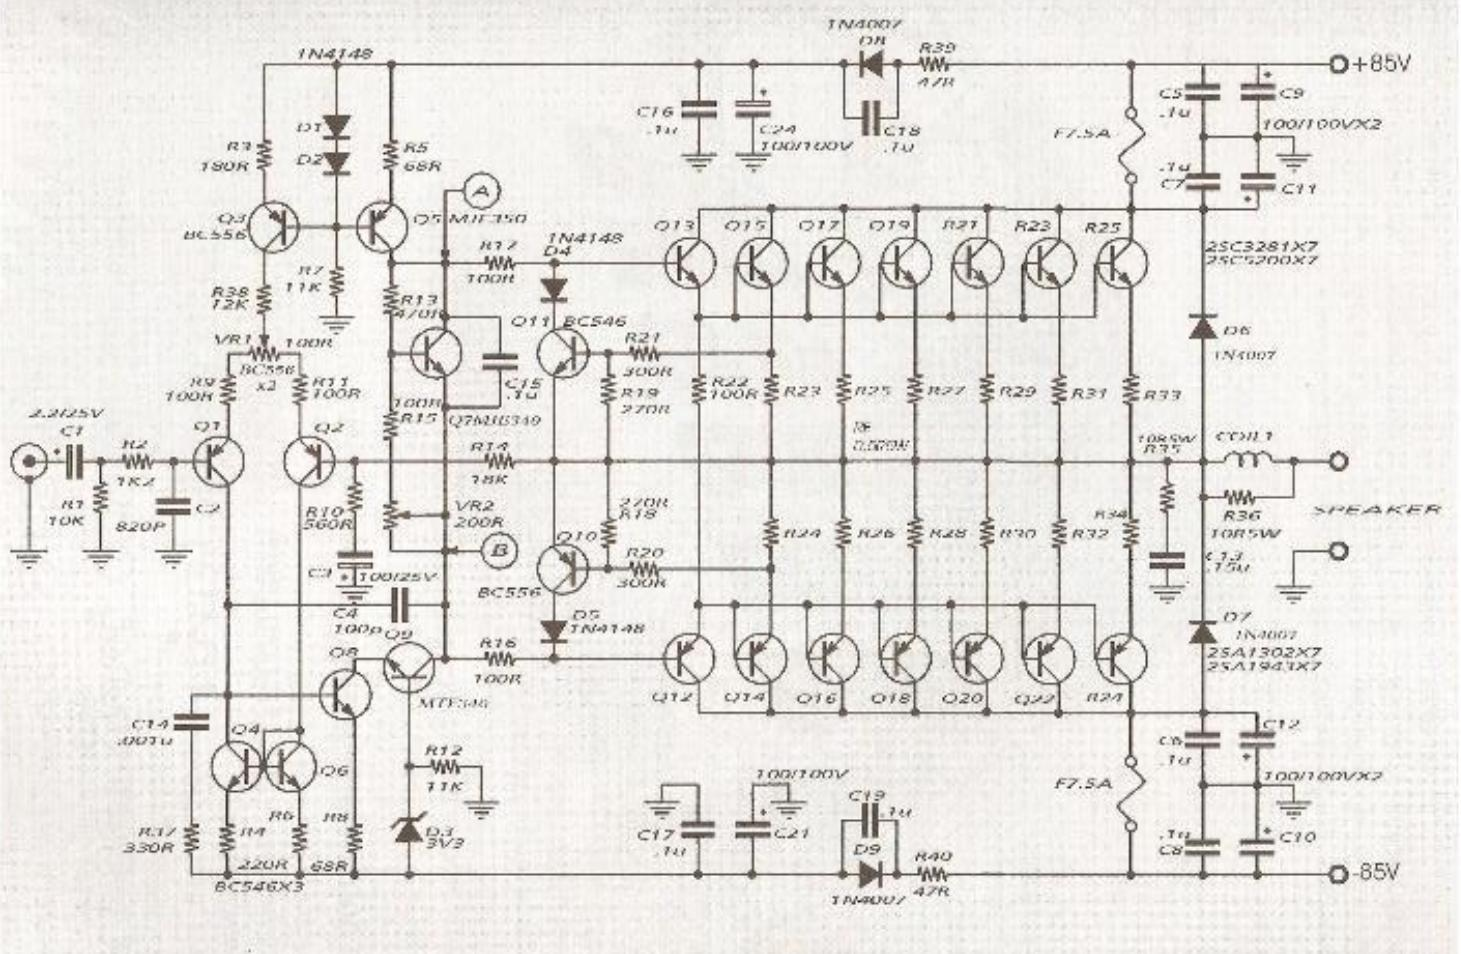
\includegraphics[keepaspectratio,
        width=\paperwidth,
        height=\paperheight]{figures/PA313_600_Circuit.jpg}
      };
    \end{tikzpicture}
  \end{frame}
}


%%--------------------------------------------------
%% Ny frame - fullscreen bild
%%--------------------------------------------------
{ % all template changes are local to this group.
  \setbeamertemplate{navigation symbols}{}
  \begin{frame}<article:0>[plain]
    \begin{tikzpicture}[remember picture,overlay]
      \node[at=(current page.center)] {
        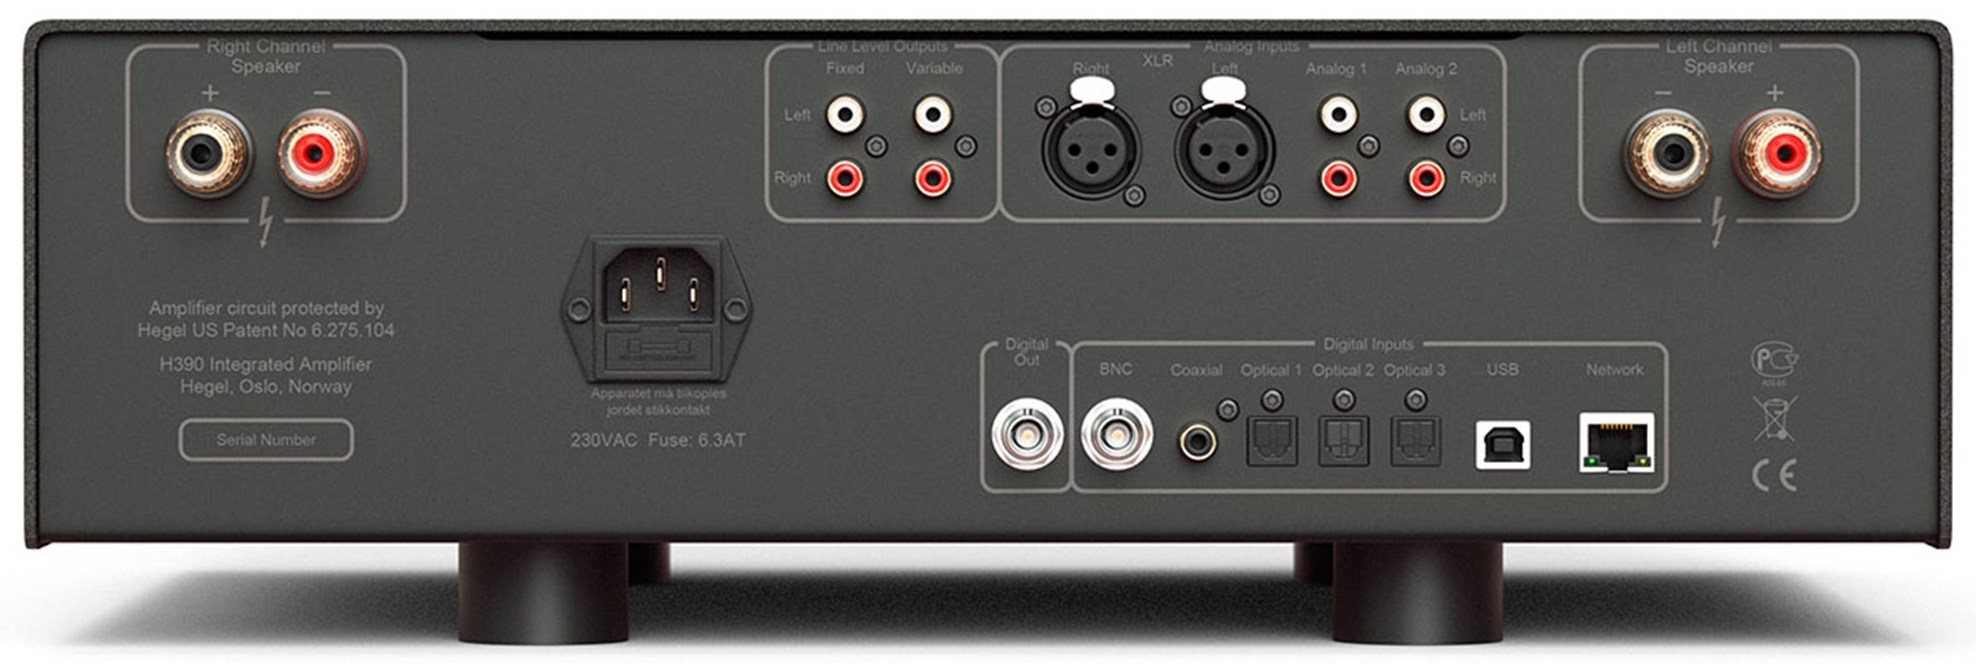
\includegraphics[keepaspectratio,
        width=\paperwidth,
        height=\paperheight]{figures/effektanpassning02.jpeg}
      };
    \end{tikzpicture}
  \end{frame}
}


%% --------------------
%% Ny frame
%% --------------------
\begin{frame}[fragile]{Effektanpassning -- spänningsdelning}
\begin{columns}
	\column{0.5\textwidth}
		\begin{circuitikz}[american]
			\draw (0,0) to[short, -*] (2,0);
			\draw (0,0) to[/tikz/circuitikz/bipoles/length=4cm,twoport, t=Hegel] (0,4);
			\draw (0,4) to[short, -*] (2,4);
			\draw (2,4) -- (4, 4)
			to[/tikz/circuitikz/bipoles/length=4cm,loudspeaker] (4,0)
			(4,0) -- (2,0);
			\node at (4,2) {B\&W};
		\end{circuitikz}
	\column{0.5\textwidth}
\end{columns}
\end{frame}


%\mode<beamer>{
%% --------------------
%% Ny frame
%% --------------------
\begin{frame}[fragile]{Effektanpassning  -- spänningsdelning}
\begin{columns}
	\column{0.5\textwidth}
		\begin{circuitikz}[american]
			\draw (0,0) to[short, -*] (2,0);
			\draw (0,0) to[vsource, invert, v=$V_t$] (0,2);
			\draw (0,2) to[R=$R_t$] (0,4);
			\draw (0,4) to[short, -*] (2,4);
			\draw (2,4) -- (4, 4)
			to[/tikz/circuitikz/bipoles/length=4cm,loudspeaker] (4,0)
			(4,0) -- (2,0);
			\node at (4,2) {B\&W};
		\end{circuitikz}
	\column{0.5\textwidth}
\end{columns}
\end{frame}
% } % end mode


%% --------------------
%% Ny frame
%% --------------------
\begin{frame}[fragile]{Effektanpassning -- spänningsdelning}
\begin{columns}
	\column{0.5\textwidth}
		\begin{circuitikz}[american]
			\node at (0,0) {};
			\draw (0.5,0) to[short, -*] (2.5,0);
			\draw (0.5,0) to[vsource, invert, v=$V_t$] (0.5,2);
			\draw (0.5,2) to[R=$R_t$] (0.5,4);
			\draw (0.5,4) to[short, -*] (2.5,4);
			\draw (2,4) -- (4, 4)
			to[R=$R_L$, i=$I_L$] (4,0)
			(4,0) -- (2,0);
		\end{circuitikz}
	\column{0.5\textwidth}
{\LARGE
		\begin{itemize}
			\item<2-> Effekt i \alert{$R_L$} är $ P_L = U_L I_L $
			\item<3-> $U_L = V_t \frac{R_L}{R_t+R_L}$
			\item<4-> $I_L = \frac{V_t}{R_t+R_L}$
			\item<5-> $P_L = V_t^2\frac{R_L}{\left(R_t+R_L\right)^2}$
			\item<6-> $P_L$ störst då $R_L = R_t$ 
		\end{itemize}
		\onslide<7->{
		\[P_{L\text{max}}=\frac{V_t^2}{4R_t}\]
		}
}
\end{columns}
\end{frame}


\handoutnoteslide


\frame{
\frametitle{}
$R_1 = \qty{68}{\kilo\ohm}$ och $R_2 = \qty{10}{\kilo\ohm}$. Beräkna $U_1$ och $U_2$.\\\vspace{5mm}
\resizebox{0.75\textwidth}{!}{%
\begin{minipage}{.5\textwidth}
\centering
  \begin{circuitikz}[american] \draw
    (0, 0) node[ground]{}
    (0, 0) to[american voltage source, invert, l=\qty{10}{V}, *-] (0,4)
    (0, 4) -- (2, 4)
    to[R=$R_2$, v=$U_2$] (2, 2)
    to[R=$R_1$, v=$U_1$] (2, 0)
    (0, 0) -- (2, 0)
    ;
  \end{circuitikz}
  \end{minipage}
}
}

\handoutnoteslide


\frame{
\frametitle{}
Koppla upp kretsen nedan. Använd samma ström för \qty{50}{\ohm}-motståndet som igår, vad skall då ställas in för $U$? Kontrollmät motstånden innan inkoppling. Mät $U_1$ och $U_2$ och säkerställ att $U=U_1+U_2$. 
\\\vspace{5mm}
\resizebox{0.75\textwidth}{!}{%
\begin{minipage}{.5\textwidth}
\centering
  \begin{circuitikz}[american] \draw
    (0, 0) node[ground]{}
    (0, 0) to[american voltage source, invert, l=$U$, *-] (0,4)
    (0, 4) -- (2, 4)
    to[R=\qty{50}{\ohm}, v=$U_2$, -*] (2, 2)
    ;
    \draw (1.5,2) -- (2.5, 2) ;
    \draw (1.5,2)
    to[R, v=$U_1$,-*] (1.5, 0) ;
    \draw (2.5, 2)
    to[R=$2 \times \qty{470}{\ohm}$] (2.5, 0) ;
    \draw (0, 0) 
        -- (2.5, 0)
    ;
  \end{circuitikz}
  \end{minipage}
}
}

\handoutnoteslide

\frame{
\frametitle{}
Koppla upp kretsen nedan. Kontrollmät motstånden innan inkoppling. Mät $U_1$ och $U_2$ och säkerställ att $U=U_1+U_2$.\\\vspace{5mm}
\resizebox{0.75\textwidth}{!}{%
\begin{minipage}{.5\textwidth}
\centering
  \begin{circuitikz}[american] \draw
    (0, 0) node[ground]{}
    (0, 0) to[american voltage source, invert, l=\qty{20}{V}, *-] (0,4)
    (0, 4) -- (2, 4)
    to[R=\qty{100}{\kohm}, v=$U_2$] (2, 2)
    to[R=\qty{100}{\kohm}, v=$U_1$] (2, 0)
    (0, 0) -- (2, 0)
    ;
  \end{circuitikz}
  \end{minipage}
}
}

\handoutnoteslide

\frame{
\frametitle{}
Koppla upp kretsen nedan. Kontrollmät motstånden innan inkoppling. Mät $U_1$ och $U_2$ och säkerställ att $U=U_1+U_2$.\\\vspace{5mm}
\resizebox{0.75\textwidth}{!}{%
\begin{minipage}{.5\textwidth}
\centering
  \begin{circuitikz}[american] \draw
    (0, 0) node[ground]{}
    (0, 0) to[american voltage source, invert, l=\qty{20}{V}, *-] (0,4)
    (0, 4) -- (2, 4)
    to[R=\qty{10}{\Mohm}, v=$U_2$] (2, 2)
    to[R=\qty{10}{\Mohm}, v=$U_1$] (2, 0)
    (0, 0) -- (2, 0)
    ;
  \end{circuitikz}
  \end{minipage}
}
}

\handoutnoteslide

\frame{
\frametitle{Så funkar ett vridspoleinstrument -- Simpson}
    {\Huge Ett mätinstrument drar ström}
}


\frame{
\frametitle{Så funkar ett vridspoleinstrument -- principen}
    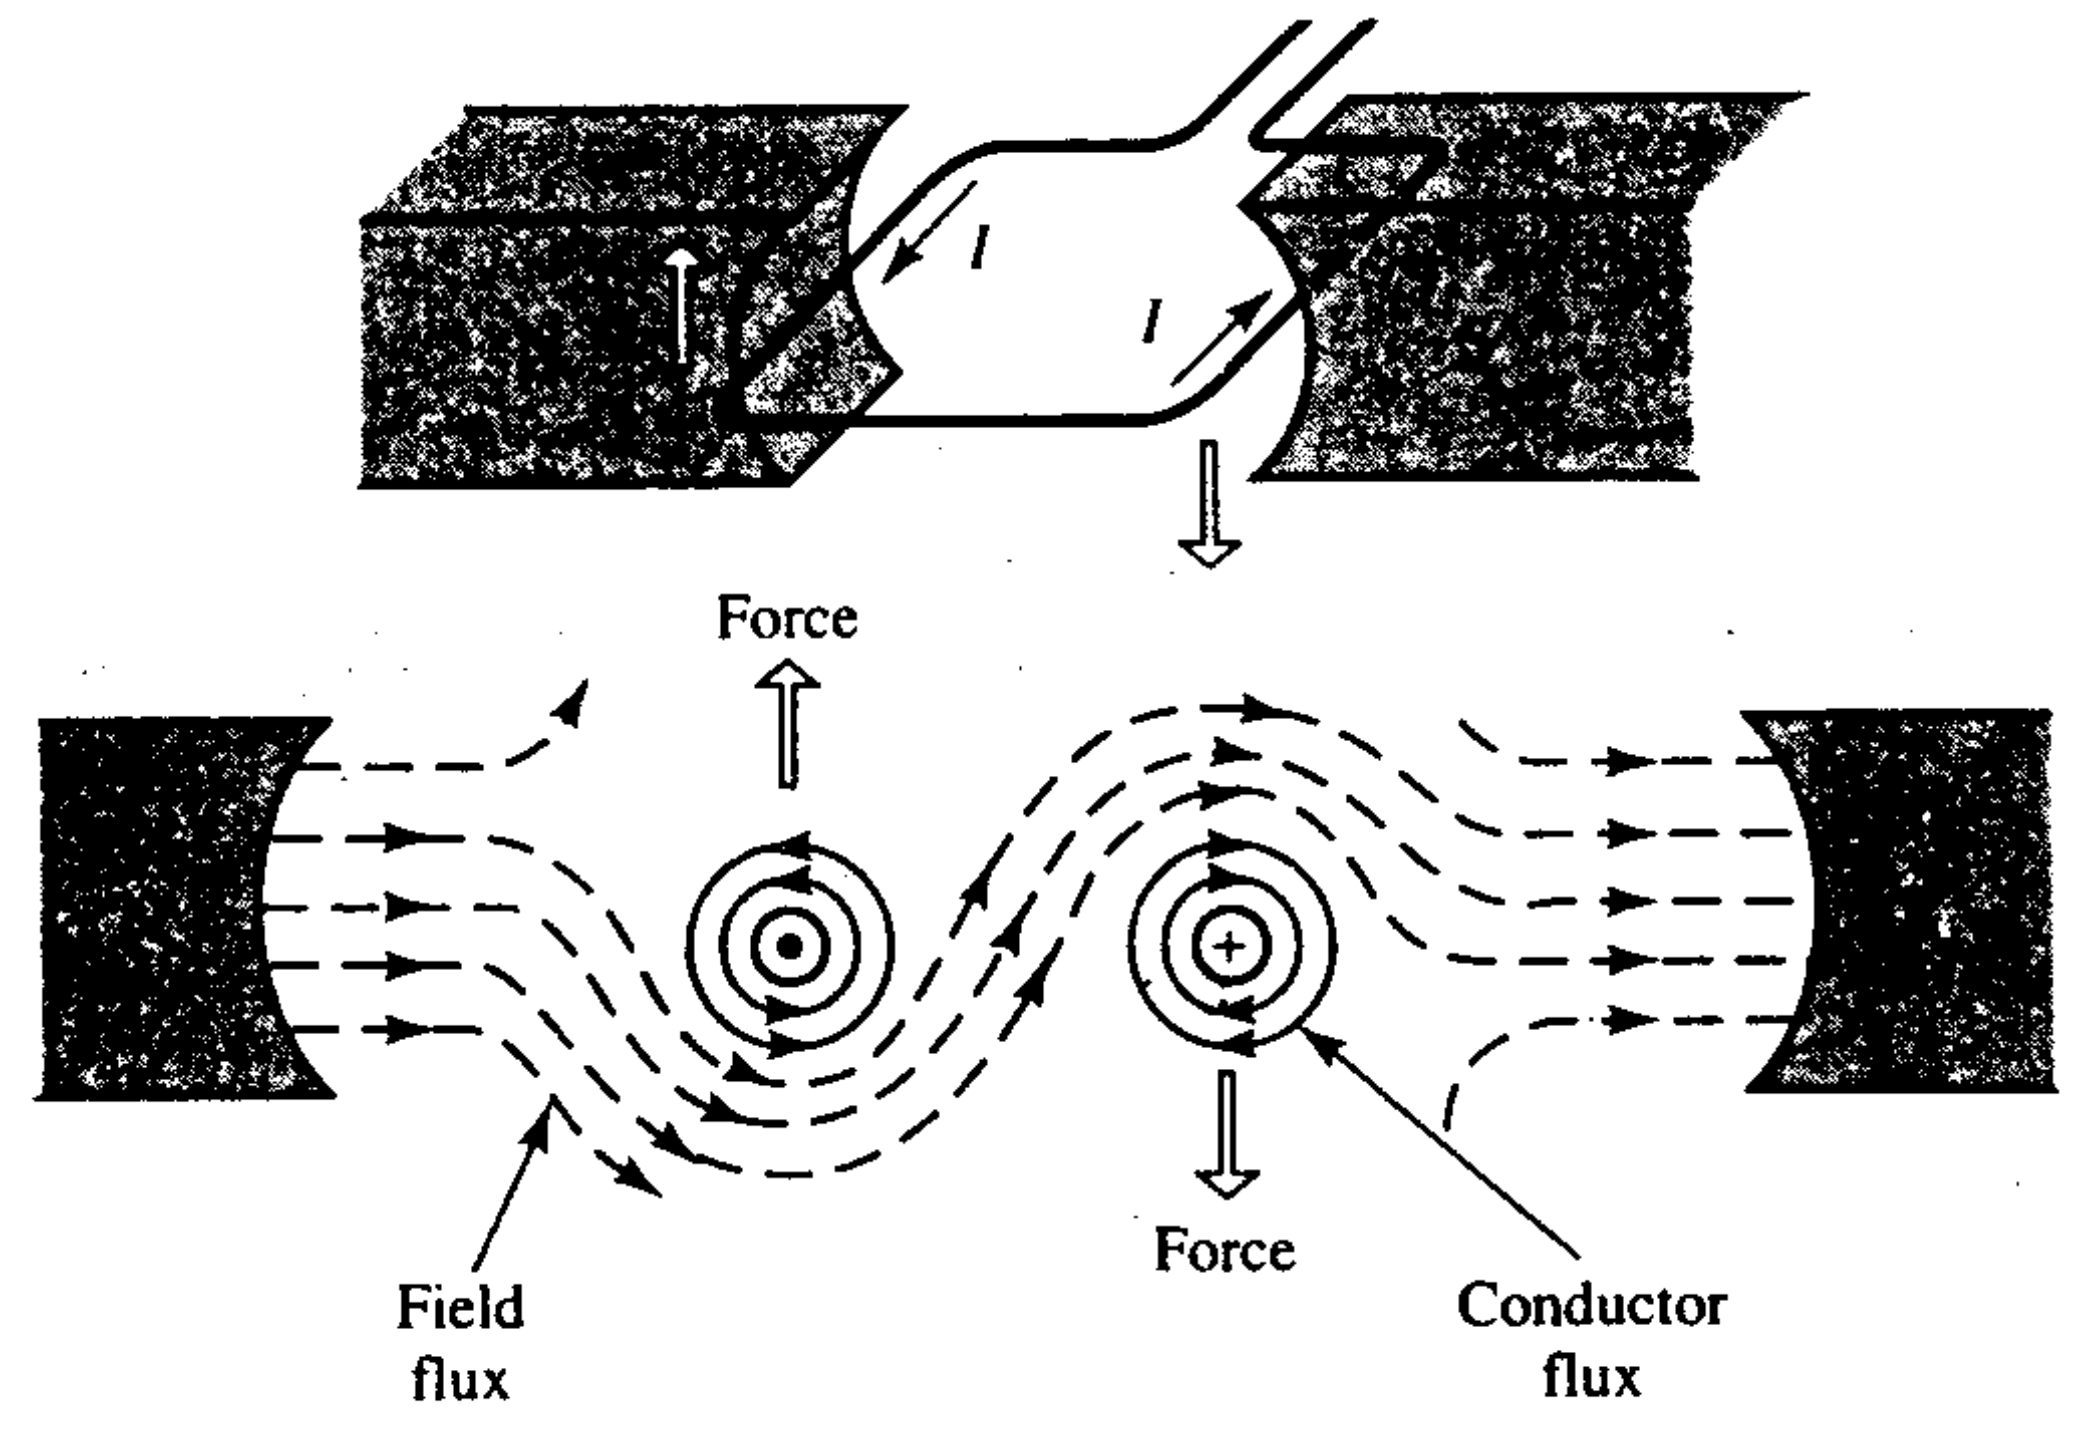
\includegraphics[width=\textwidth]{figures/stromslinga_i_magnetfalt.png}
}


\frame{
\frametitle{Så funkar ett vridspoleinstrument -- ingnejörskonsten}
    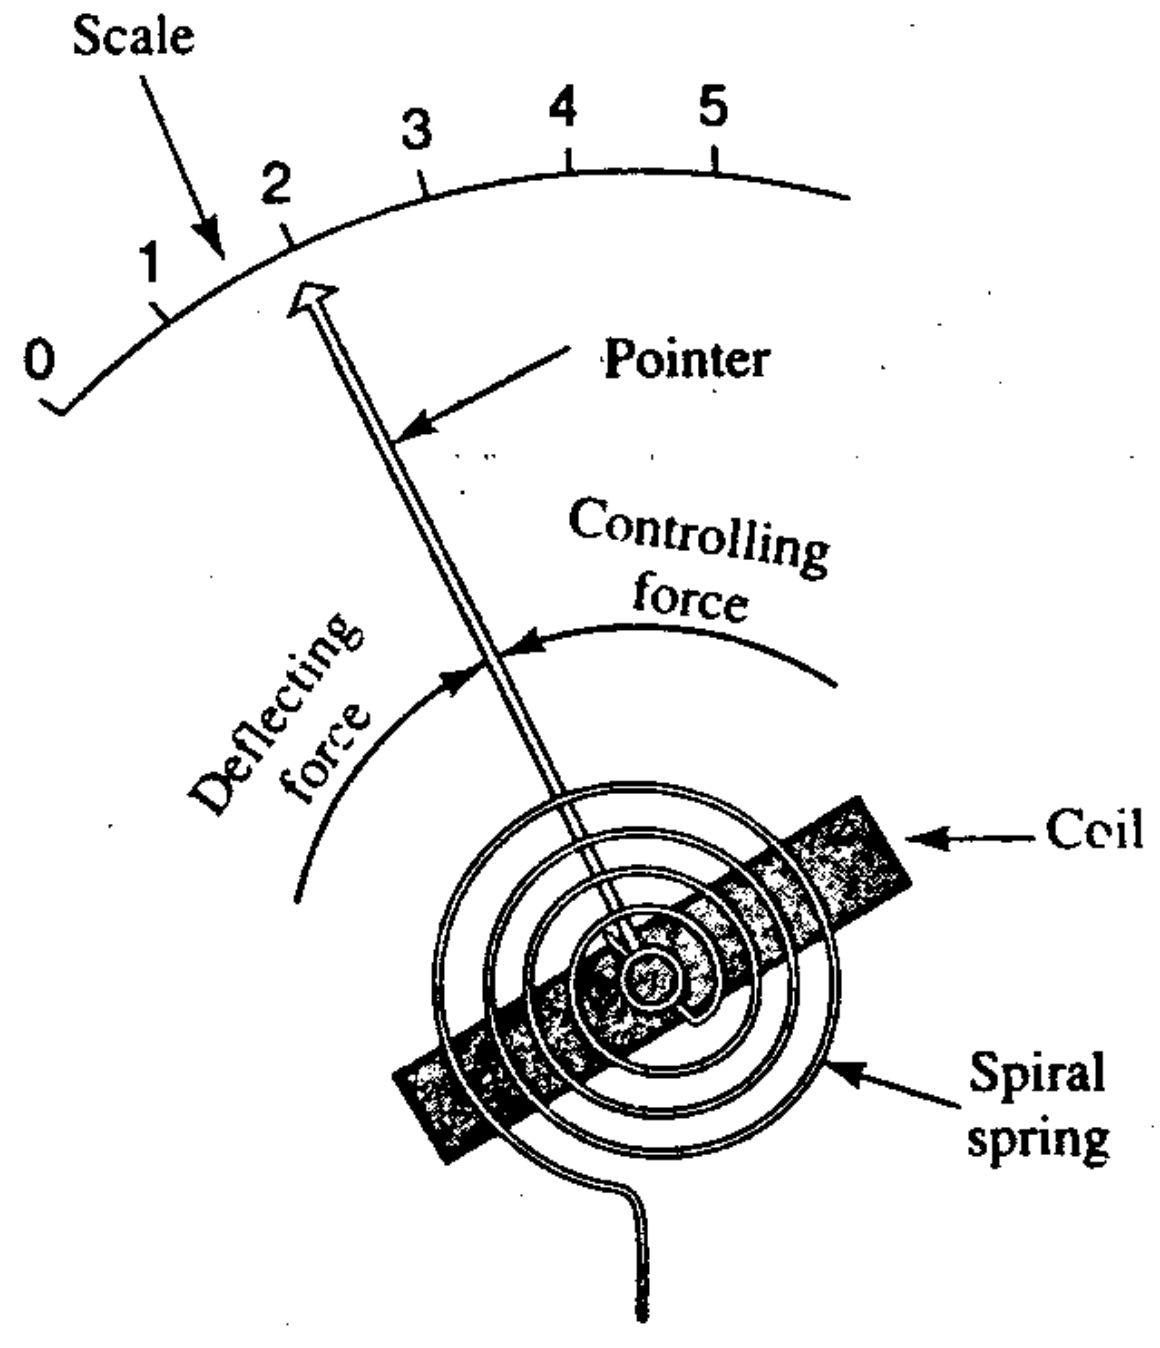
\includegraphics[width=0.45\textwidth]{figures/pmmc.png}
    \onslide<2->{
    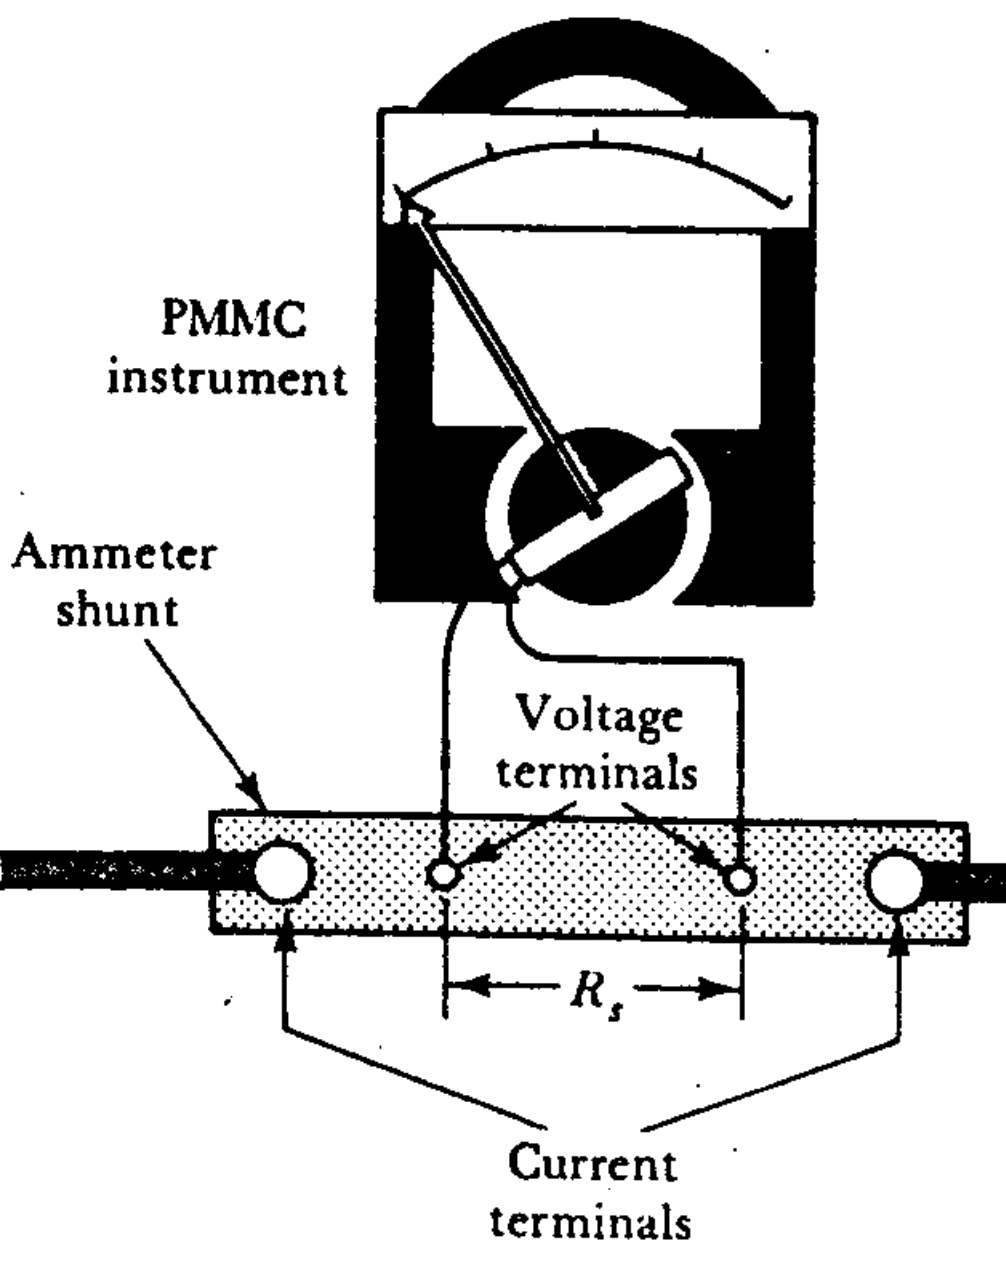
\includegraphics[width=0.45\textwidth]{figures/pmmc_instrument.png}
    }
}


\frame{
\frametitle{Så funkar ett vridspoleinstrument -- kretsen}
    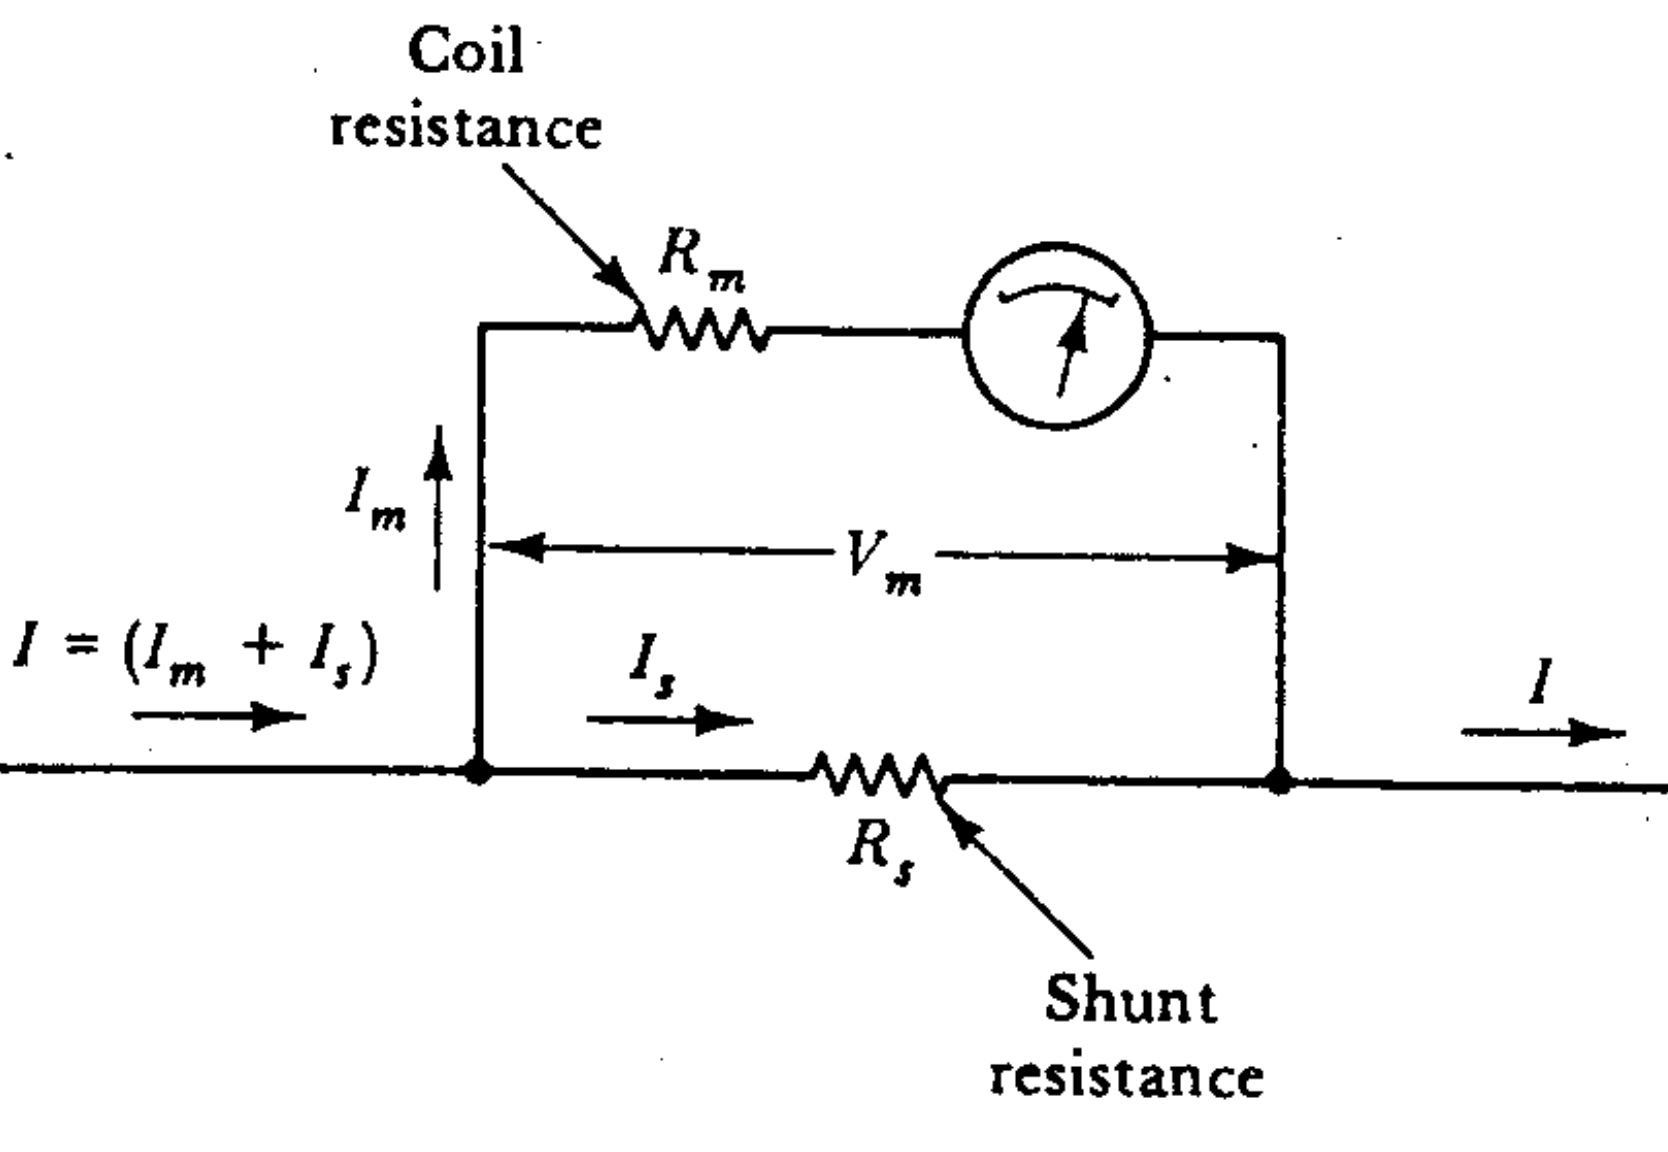
\includegraphics[width=0.85\textwidth]{figures/pmmc_circuit.png}
}


\frame{
\frametitle{Så funkar ett vridspoleinstrument -- flera mätområden}
    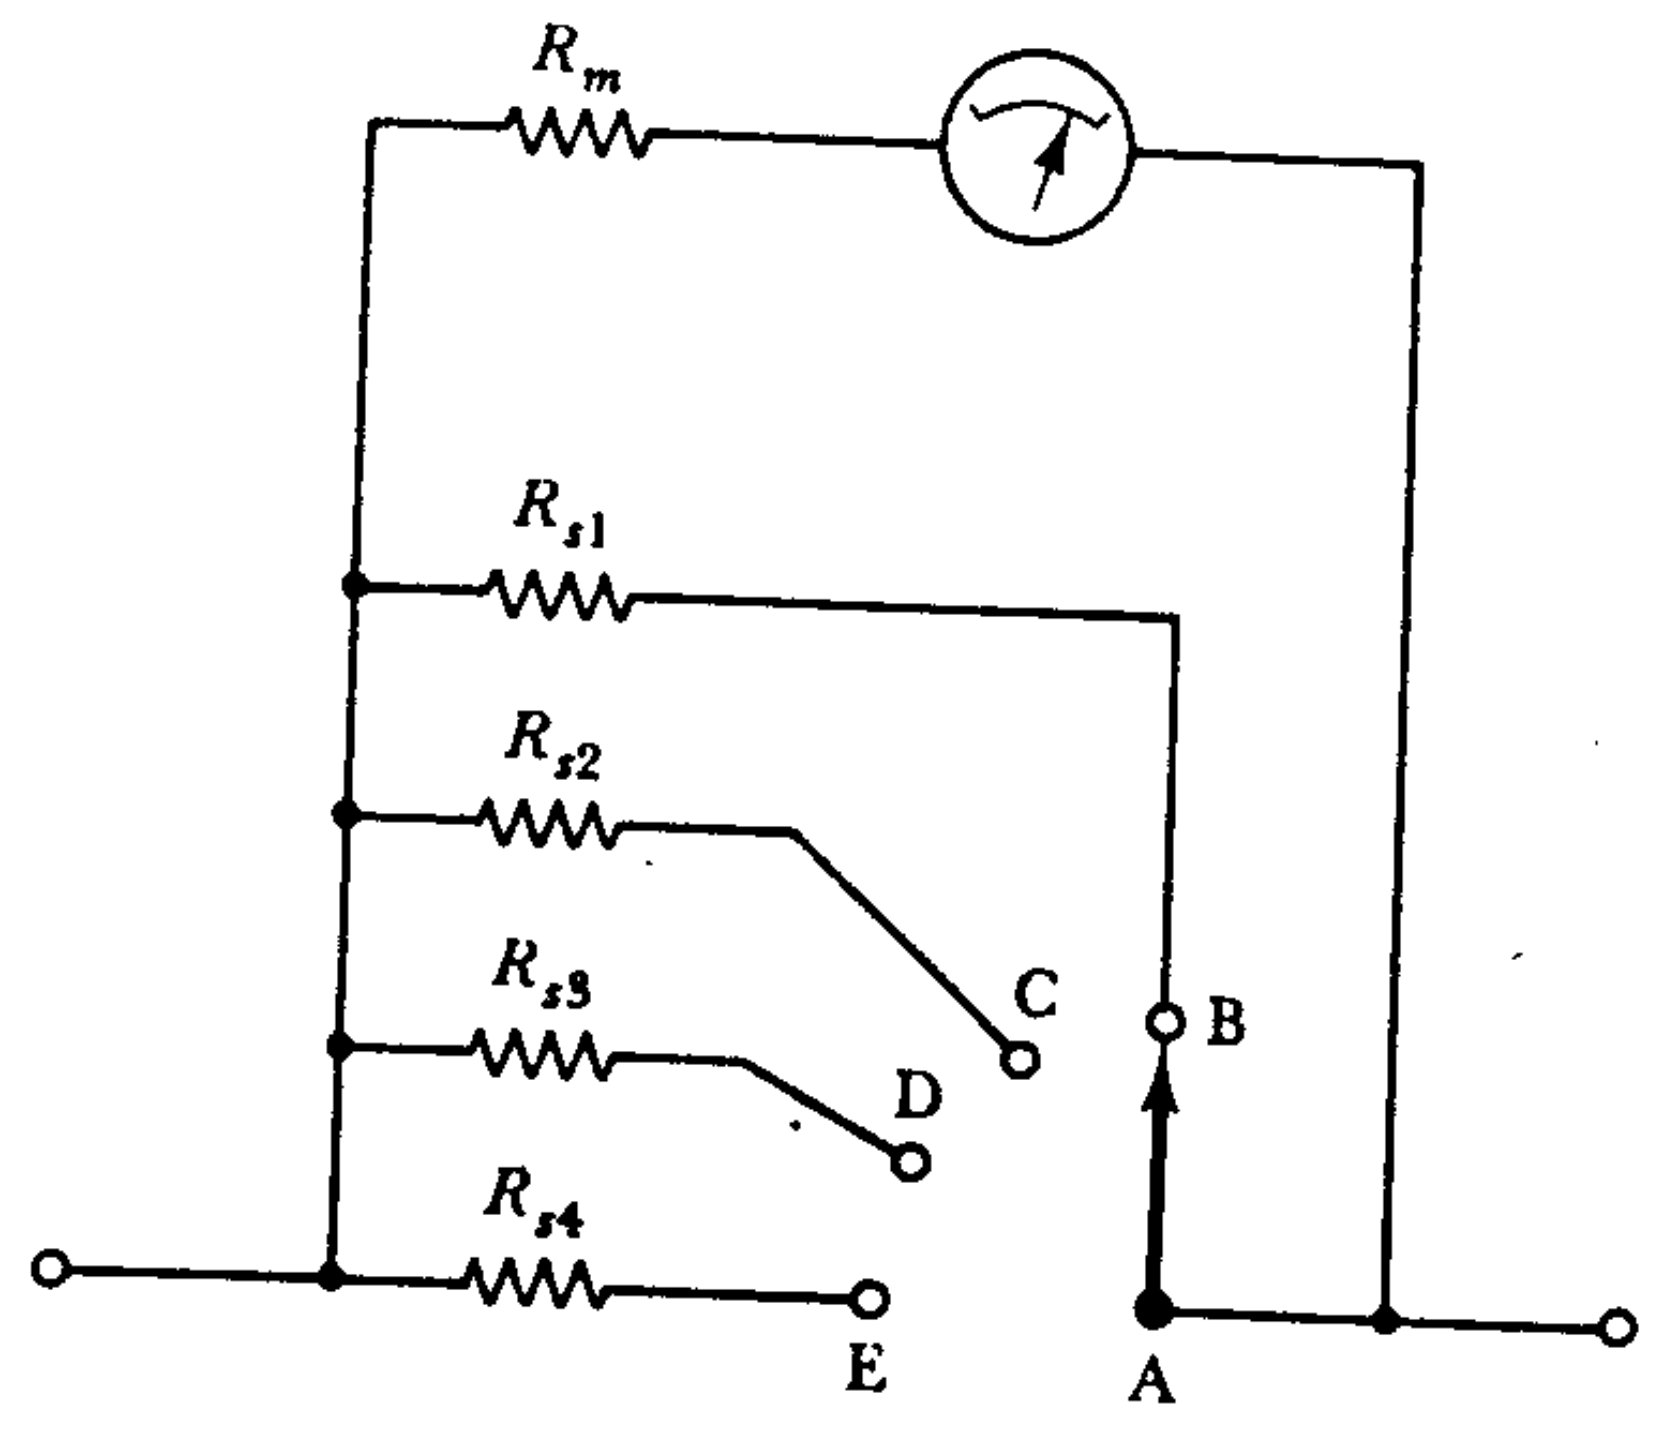
\includegraphics[height=0.9\textheight, angle=2.5]{figures/pmmc_multirange.png}
}


\frame{
\frametitle{Så funkar ett digitalt instrument}
    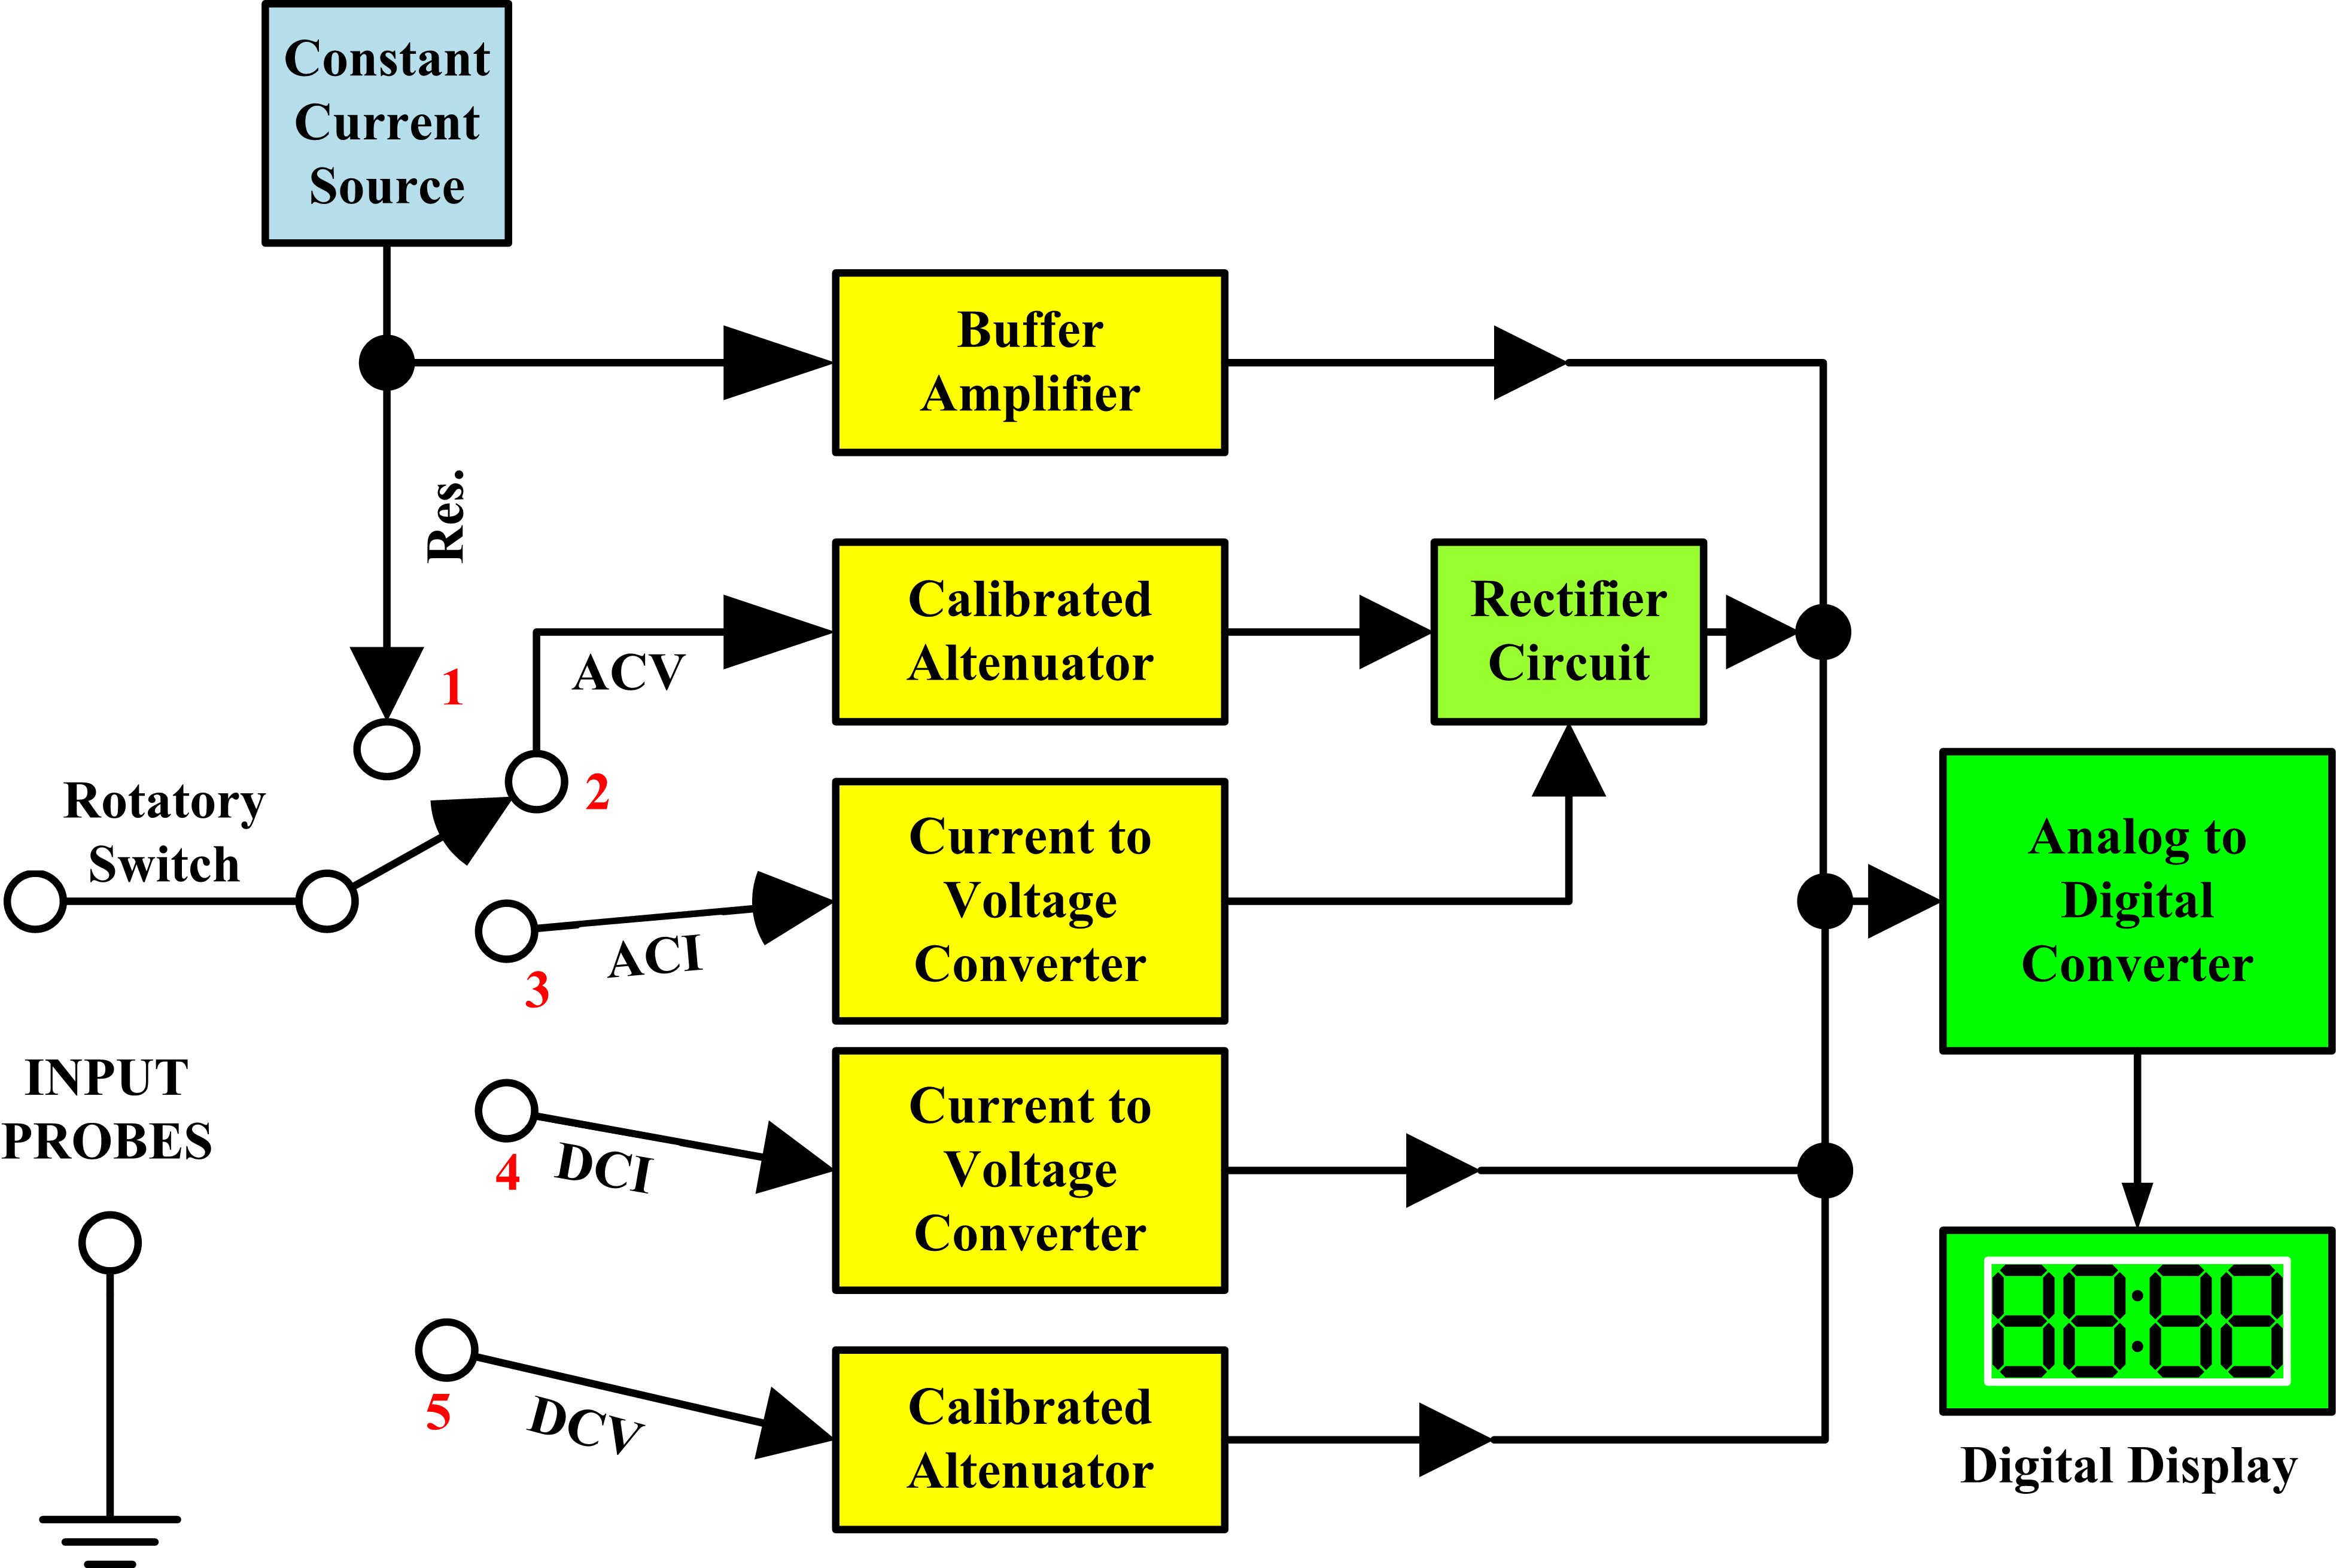
\includegraphics[width=0.85\textwidth, angle=0]{figures/dmm_skiss.png}
}


\frame{
\frametitle{Modell (för räkning och förståelse) av instrument}
\centering
{\huge Inre resistans i instrument!}\\
\vspace{5mm}
\resizebox{\textwidth}{!}{%
\begin{minipage}{.5\textwidth}
\centering
  \begin{circuitikz}[american] \draw
    (0, 0) 
    to[voltmeter] (0, 2)
    to[short, -o] (2, 2)
    ;
    \draw (0, 0)
    to[short, -o] (2, 0)
    ;
    \draw (1, 2)
    to[R=$R_V$, *-*] (1, 0)
    ;
    \node[anchor = north] at (1, 0) {Voltmeter} ;
    \draw
    (0+3, 0) 
    to[ammeter] (0+3, 2)
    to[R,l_=$R_A$, -o] (2+3, 2)
    ;
    \draw (0+3, 0)
    to[short, -o] (2+3, 0)
    ;
%    \draw (1+3, 2)
%    to[R=$R_V$, *-*] (1+3, 0)
%    ;
    \node[anchor = north] at (1+3, 0) {Amperemeter} ;
    
  \end{circuitikz}
  \end{minipage}
}
}

\handoutnoteslide

\frame{
\frametitle{Inre resistans}
{\huge
\begin{itemize}
    \item Mät inre resistansen i ert instrument!
    \item Räkna (med spänningsdelning!) vad just din multimeter borde visat vid mätning av \qty{10}{\Mohm}-delningen.
\end{itemize}
}
}

\handoutnoteslide

\frame{
\frametitle{Intre resistans -- amperemätning}
\resizebox{\textwidth}{!}{%
\begin{minipage}{.75\textwidth}
\centering
  \begin{circuitikz}[american] \draw
    (0, 0) 
    to[american voltage source=\qty{1}{\V}, invert] (0, 2)
    to[ammeter] (2, 2)
    to[R=\qty{10}{\ohm}] (2, 0)
    -- (0,0)
    ;
      \end{circuitikz}
  \end{minipage}
}
{\Large
\begin{itemize}
    \item Mät ström \unit{\mA}-ingång.
    \item Koppla i och ur amperemetern.
    \item Betrakta strömmen på \emph{spänningskuben}.
    \item Beräkna $R_A$.
\end{itemize}
}
}

\handoutnoteslide

\frame{
\frametitle{}
{\Huge 
Lite om statisk elektricitet
}
}

\frame{
    \frametitle{}
    \begin{tikzpicture}[remember picture,overlay]
        \node[at=(current page.center)] {
            
\includegraphics[keepaspectratio,
                                 width=\paperwidth,
                                 height=\paperheight]{figures/static.jpg}
            };
    \end{tikzpicture}    
    }

\frame{
\frametitle{\textbf{Lika} laddningar repellerar}
\resizebox{\textwidth}{!}{%
\begin{minipage}{.6\textwidth}
\centering
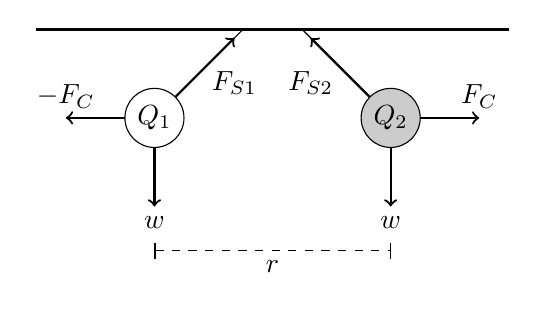
\begin{tikzpicture}[scale=0.75]
			% Left charge
			\draw (0,0) -- (15mm,15mm) ;
			\fill[white] (0,0) circle (5mm) ;
			\draw (0,0) circle (5mm) ;
			\draw (0,0) node[] {$Q_1$} ;
			\draw[thick,->] (0,0) ++ (-5mm,0) -- + (-10mm,0) coordinate (leftF);
			\draw (leftF) node[anchor= south] {$-F_C$} ;
			\draw[thick,->] (0,0) ++ (0,-5mm) -- + (0,-10mm) coordinate (q1downF);
			\draw (q1downF) node[anchor= north] {$w$} ;
			\draw[thick,->] (0,0) ++ (3.54mm, 3.54mm) -- + (10mm, 10mm) coordinate (leftFs) ;
			\draw (leftFs) ++ (0,-4mm) node[anchor= north] {$F_{S1}$} ;
			% Right charge
			\draw (4,0) -- + (-15mm,15mm) ;
			\fill[gray!40!white] (4,0) circle (5mm) ;
			\draw (4,0) circle (5mm) ;
			\draw (4,0) node[] {$Q_2$} ;
			\draw[thick,->] (4,0) ++ (5mm,0) -- + (10mm,0) coordinate (rightF);
			\draw (rightF) node[anchor= south] {$F_C$} ;
			\draw[thick,->] (4,0) ++ (0,-5mm) -- + (0,-10mm) coordinate (q2downF);
			\draw (q2downF) node[anchor= north] {$w$} ;
			\draw[thick,->] (4,0) ++ (-3.54mm, 3.54mm) -- + (-10mm, 10mm) coordinate (rightFs) ;
			\draw (rightFs) ++ (0,-4mm) node[anchor= north] {$F_{S2}$} ;
			% Roof and coordinate r
			\draw[very thick] (-2,1.5) -- (6,1.5) ;
			\draw[|-|, dashed] (0,-2.25) -- (4, -2.25) ;
			\draw (2,-2.25) node[anchor = north] {$r$};
		\end{tikzpicture}
  \end{minipage}
}
}

\frame{
\frametitle{\textbf{Olika} laddningar attraherar}
\resizebox{\textwidth}{!}{%
\begin{minipage}{.6\textwidth}
\centering
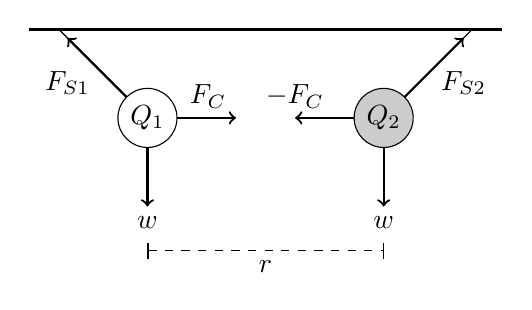
\begin{tikzpicture}[scale=0.75]
				% Left charge
				\draw (0,0) -- (-15mm,15mm) ;
				\fill[white] (0,0) circle (5mm) ;
				\draw (0,0) circle (5mm) ;
				\draw (0,0) node[] {$Q_1$} ;
				\draw[thick,->] (0,0) ++ (5mm,0) -- + (10mm,0) coordinate (leftF);
				\draw (leftF) node[anchor= south east] {$F_C$} ;
				\draw[thick,->] (0,0) ++ (0,-5mm) -- + (0,-10mm) coordinate (q1downF);
				\draw (q1downF) node[anchor= north] {$w$} ;
				\draw[thick,->] (0,0) ++ (-3.54mm, 3.54mm) -- + (-10mm, 10mm) coordinate (leftFs) ;
				\draw (leftFs) ++ (0,-4mm) node[anchor= north] {$F_{S1}$} ;
				% Right charge
				\draw (4,0) -- + (15mm,15mm) ;
				\fill[gray!40!white] (4,0) circle (5mm) ;
				\draw (4,0) circle (5mm) ;
				\draw (4,0) node[] {$Q_2$} ;
				\draw[thick,->] (4,0) ++ (-5mm,0) -- + (-10mm,0) coordinate (rightF);
				\draw (rightF) node[anchor= south] {$-F_C$} ;
				\draw[thick,->] (4,0) ++ (0,-5mm) -- + (0,-10mm) coordinate (q2downF);
				\draw (q2downF) node[anchor= north] {$w$} ;
				\draw[thick,->] (4,0) ++ (3.54mm, 3.54mm) -- + (10mm, 10mm) coordinate (rightFs) ;
				\draw (rightFs) ++ (0,-4mm) node[anchor= north] {$F_{S2}$} ;
				% Roof and coordinate r
				\draw[very thick] (-2,1.5) -- (6,1.5) ;
				\draw[|-|, dashed] (0,-2.25) -- (4, -2.25) ;
				\draw (2,-2.25) node[anchor = north] {$r$};
			\end{tikzpicture}
  \end{minipage}
}
}


%%--------------------------------------------------
%% Ny frame
%%--------------------------------------------------
\begin{frame}[fragile]{Kondensatorn}
  
%  \vspace{5mm}
  \begin{columns}
    \column{0.7\textwidth}
        \begin{itemize}
      \item Sparar energi $\Rightarrow$ omfördela laddningar
        på \alert{kondensatorn}
      \item<2-> Kondensatorns \alert{kapacitans} def:
        \[C=\frac{Q}{U}\onslide<3->{\Rightarrow Q=C \cdot{} U}\]
       \onslide<4->{ (enhet Farad --
         $\qty{1}{\farad}=\qty{1}{\per\kg\per\square\metre\second\tothe{4}\ampere\squared}$)
       }
     \item<5-> Större ytor $\Rightarrow$ fler laddningar
     \item<6-> Tätare plattor $\Rightarrow$ laddningar attraheras
      \end{itemize}
       \begin{columns}
         \column{0.5\textwidth}
                \onslide<7-> {\[C=\frac{A\varepsilon_0\varepsilon_r}{d}\]}
       \onslide<8->{ \alert{Luft mellan plattorna} $\varepsilon_r=1$}

       \column{0.5\textwidth}
             \onslide<9->{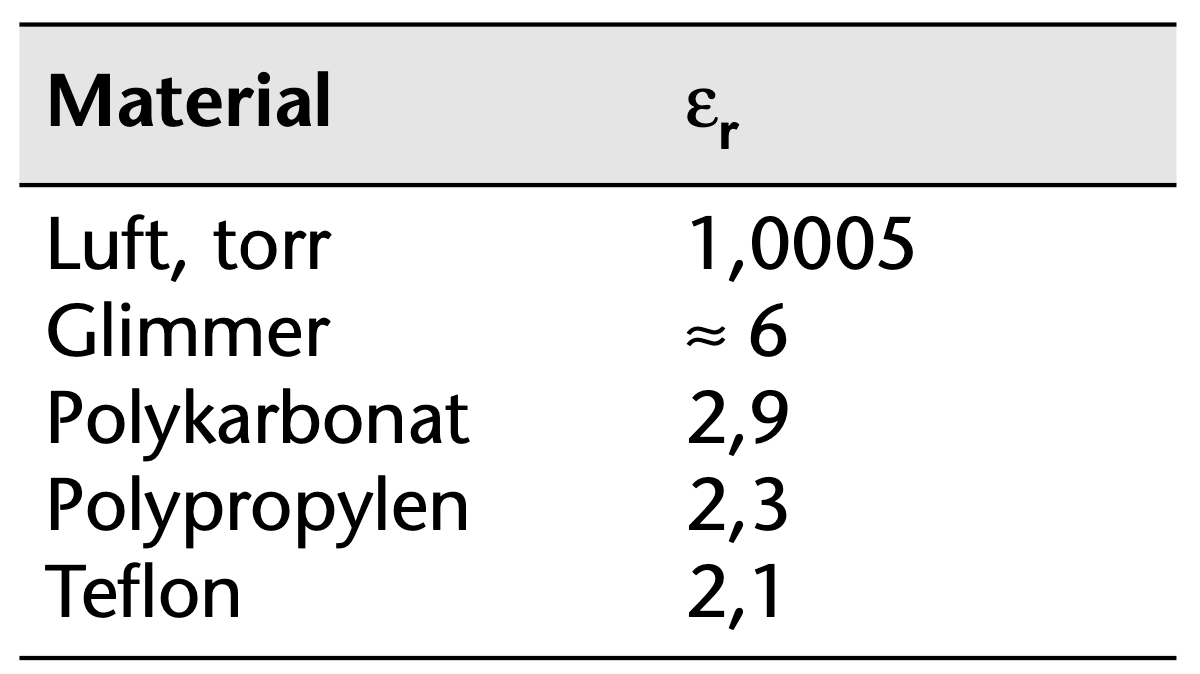
\includegraphics[width =
        \textwidth]{figures/epsilontabell.png}}
       \end{columns}
       


      \column{0.3\textwidth}
      \onslide<1->{
      %\includegraphics[width = 0.6\textwidth]{figures/kondensator.png}
      	      	\begin{tikzpicture}
	\draw (0, 0) to[C=$C_1$, o-o] (2, 0) ;
	\end{tikzpicture}\\\vspace{2mm}}
\onslide<5->{
      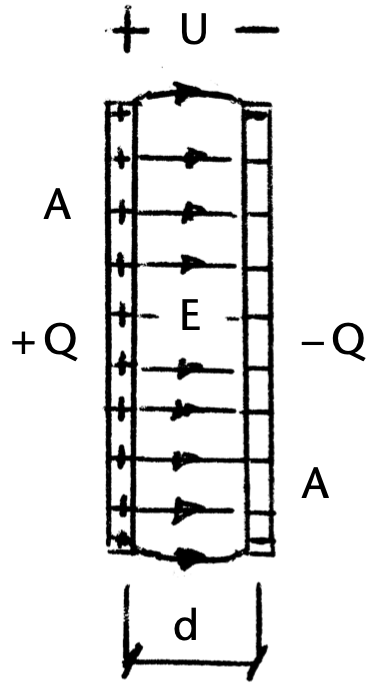
\includegraphics[width =
      0.7\textwidth]{figures/plattkond.png}}
    \end{columns}
    \begin{center}
      \end{center}
\end{frame}


\handoutnoteslide


%%% --------------------
%%% Ny frame
%%% --------------------
%\begin{frame}[fragile]{Effektanpassning}
%\begin{columns}
%	\column{0.5\textwidth}
%	\column{0.5\textwidth}
%\end{columns}
%\end{frame}
%
%
%%--------------------------------------------------
%% Ny frame
%%--------------------------------------------------
\begin{frame}[fragile]{Kapacitans -- exempel}
  \begin{columns}
    \column{0.3\textwidth}
    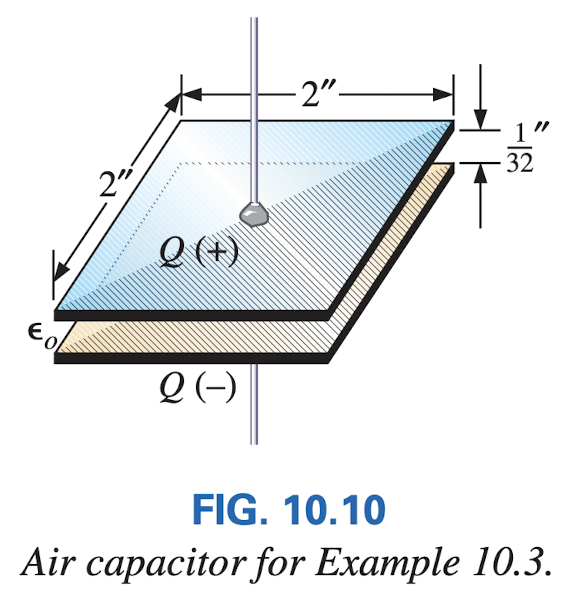
\includegraphics[width = \textwidth]{figures/plattkondex.png}
    \column{0.7\textwidth}
    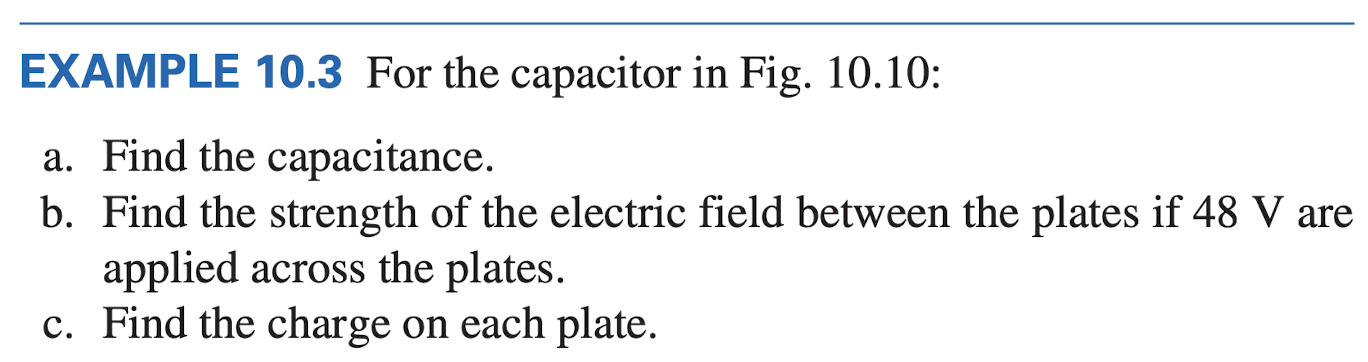
\includegraphics[width = \textwidth]{figures/plattkondex_text.png}
  \end{columns}
  \begin{columns}
    \column{0.3\textwidth}
      \onslide<2->{
      \[C=\frac{A\varepsilon_0\varepsilon_r}{d}\]
    }
    \onslide<2->{
      \[C=\frac{Q}{U}\onslide<3->{\Rightarrow Q=C \cdot{} U}\]
    }
    \column{0.7\textwidth}
  \end{columns}
  \vspace{30mm}
\end{frame}

\handoutnoteslide

%%--------------------------------------------------
%% Ny frame
%%--------------------------------------------------
\begin{frame}[fragile]{Kondensatorer i kretsar}
  \begin{columns}
    \column{0.67\textwidth}
    \begin{itemize}
    \item Batteri laddar upp kondensator
    \item<2-> \alert{OBS} elektrolytkond \alert{rätt håll!}
    \end{itemize}
    \begin{columns}
      \column{0.5\textwidth}
      \onslide<3->{
        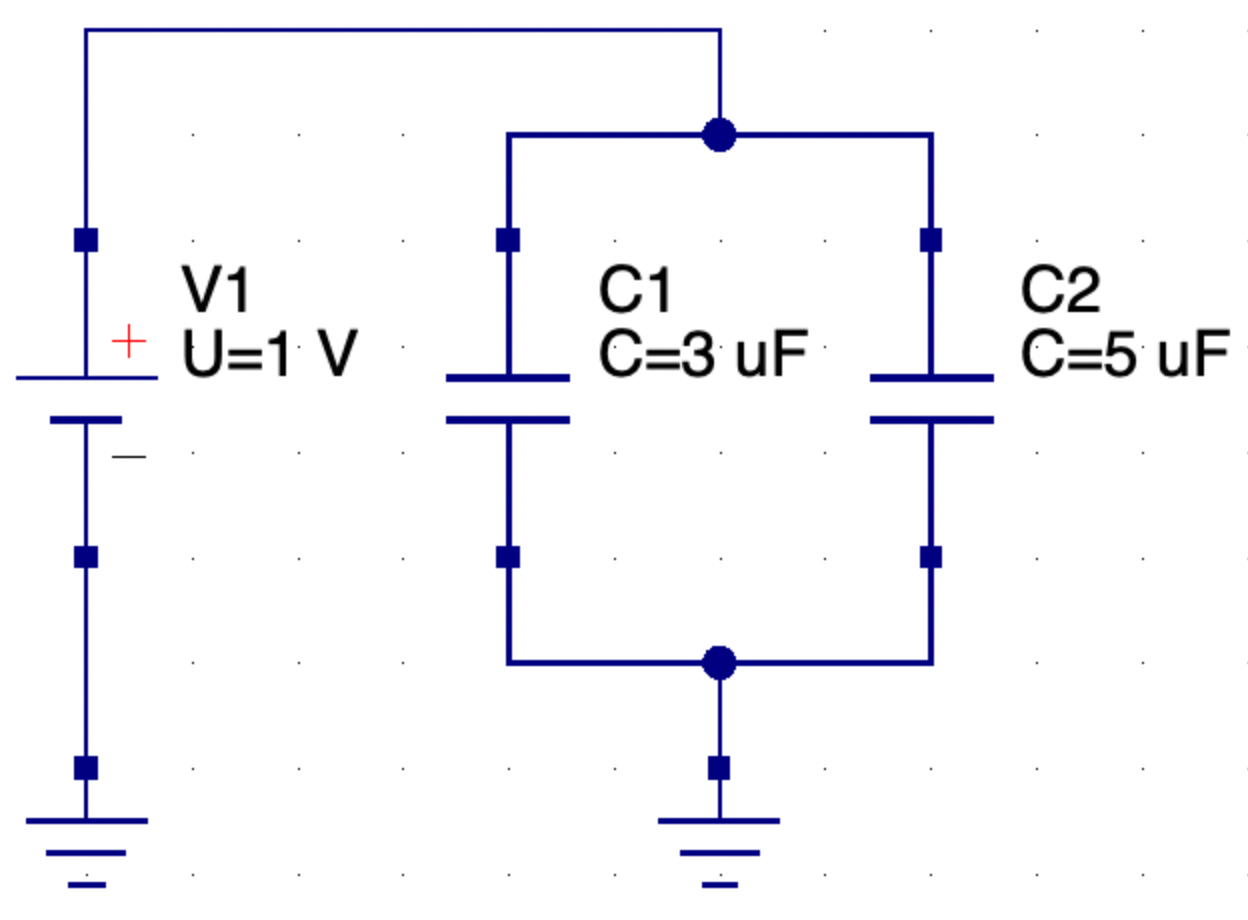
\includegraphics[width = 0.75\textwidth]{figures/kondparallell.png}\\
        Parallella $\Rightarrow$ högre kapacitans!
        \[C_\mathrm{tot}=C3+C4+\ldots\]
      }
      \column{0.5\textwidth}
      \onslide<4->{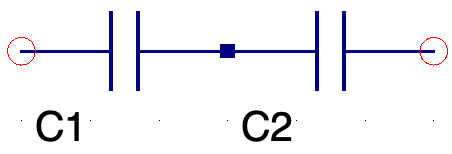
\includegraphics[width = \textwidth]{figures/kondserie.png}\\
        Serie $\Rightarrow$ lägre kapacitans!
        \[\frac{1}{C_\mathrm{tot}}=\frac{1}{C1}+\frac{1}{C2}+\ldots\]
      }
    \end{columns}
    \column{0.33\textwidth}
    \onslide<1->{
      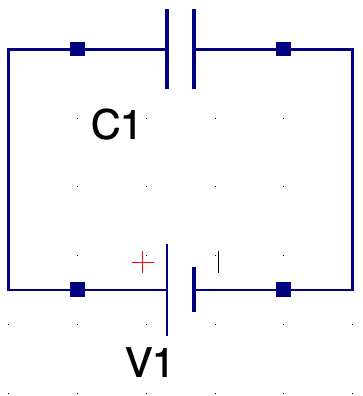
\includegraphics[width=0.75\textwidth]{figures/kondkrets.png}
    } \\
    \onslide<1->{
      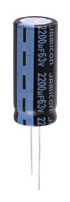
\includegraphics[width = 0.30\textwidth]{figures/konding.jpg}
    }
    \onslide<1->{
      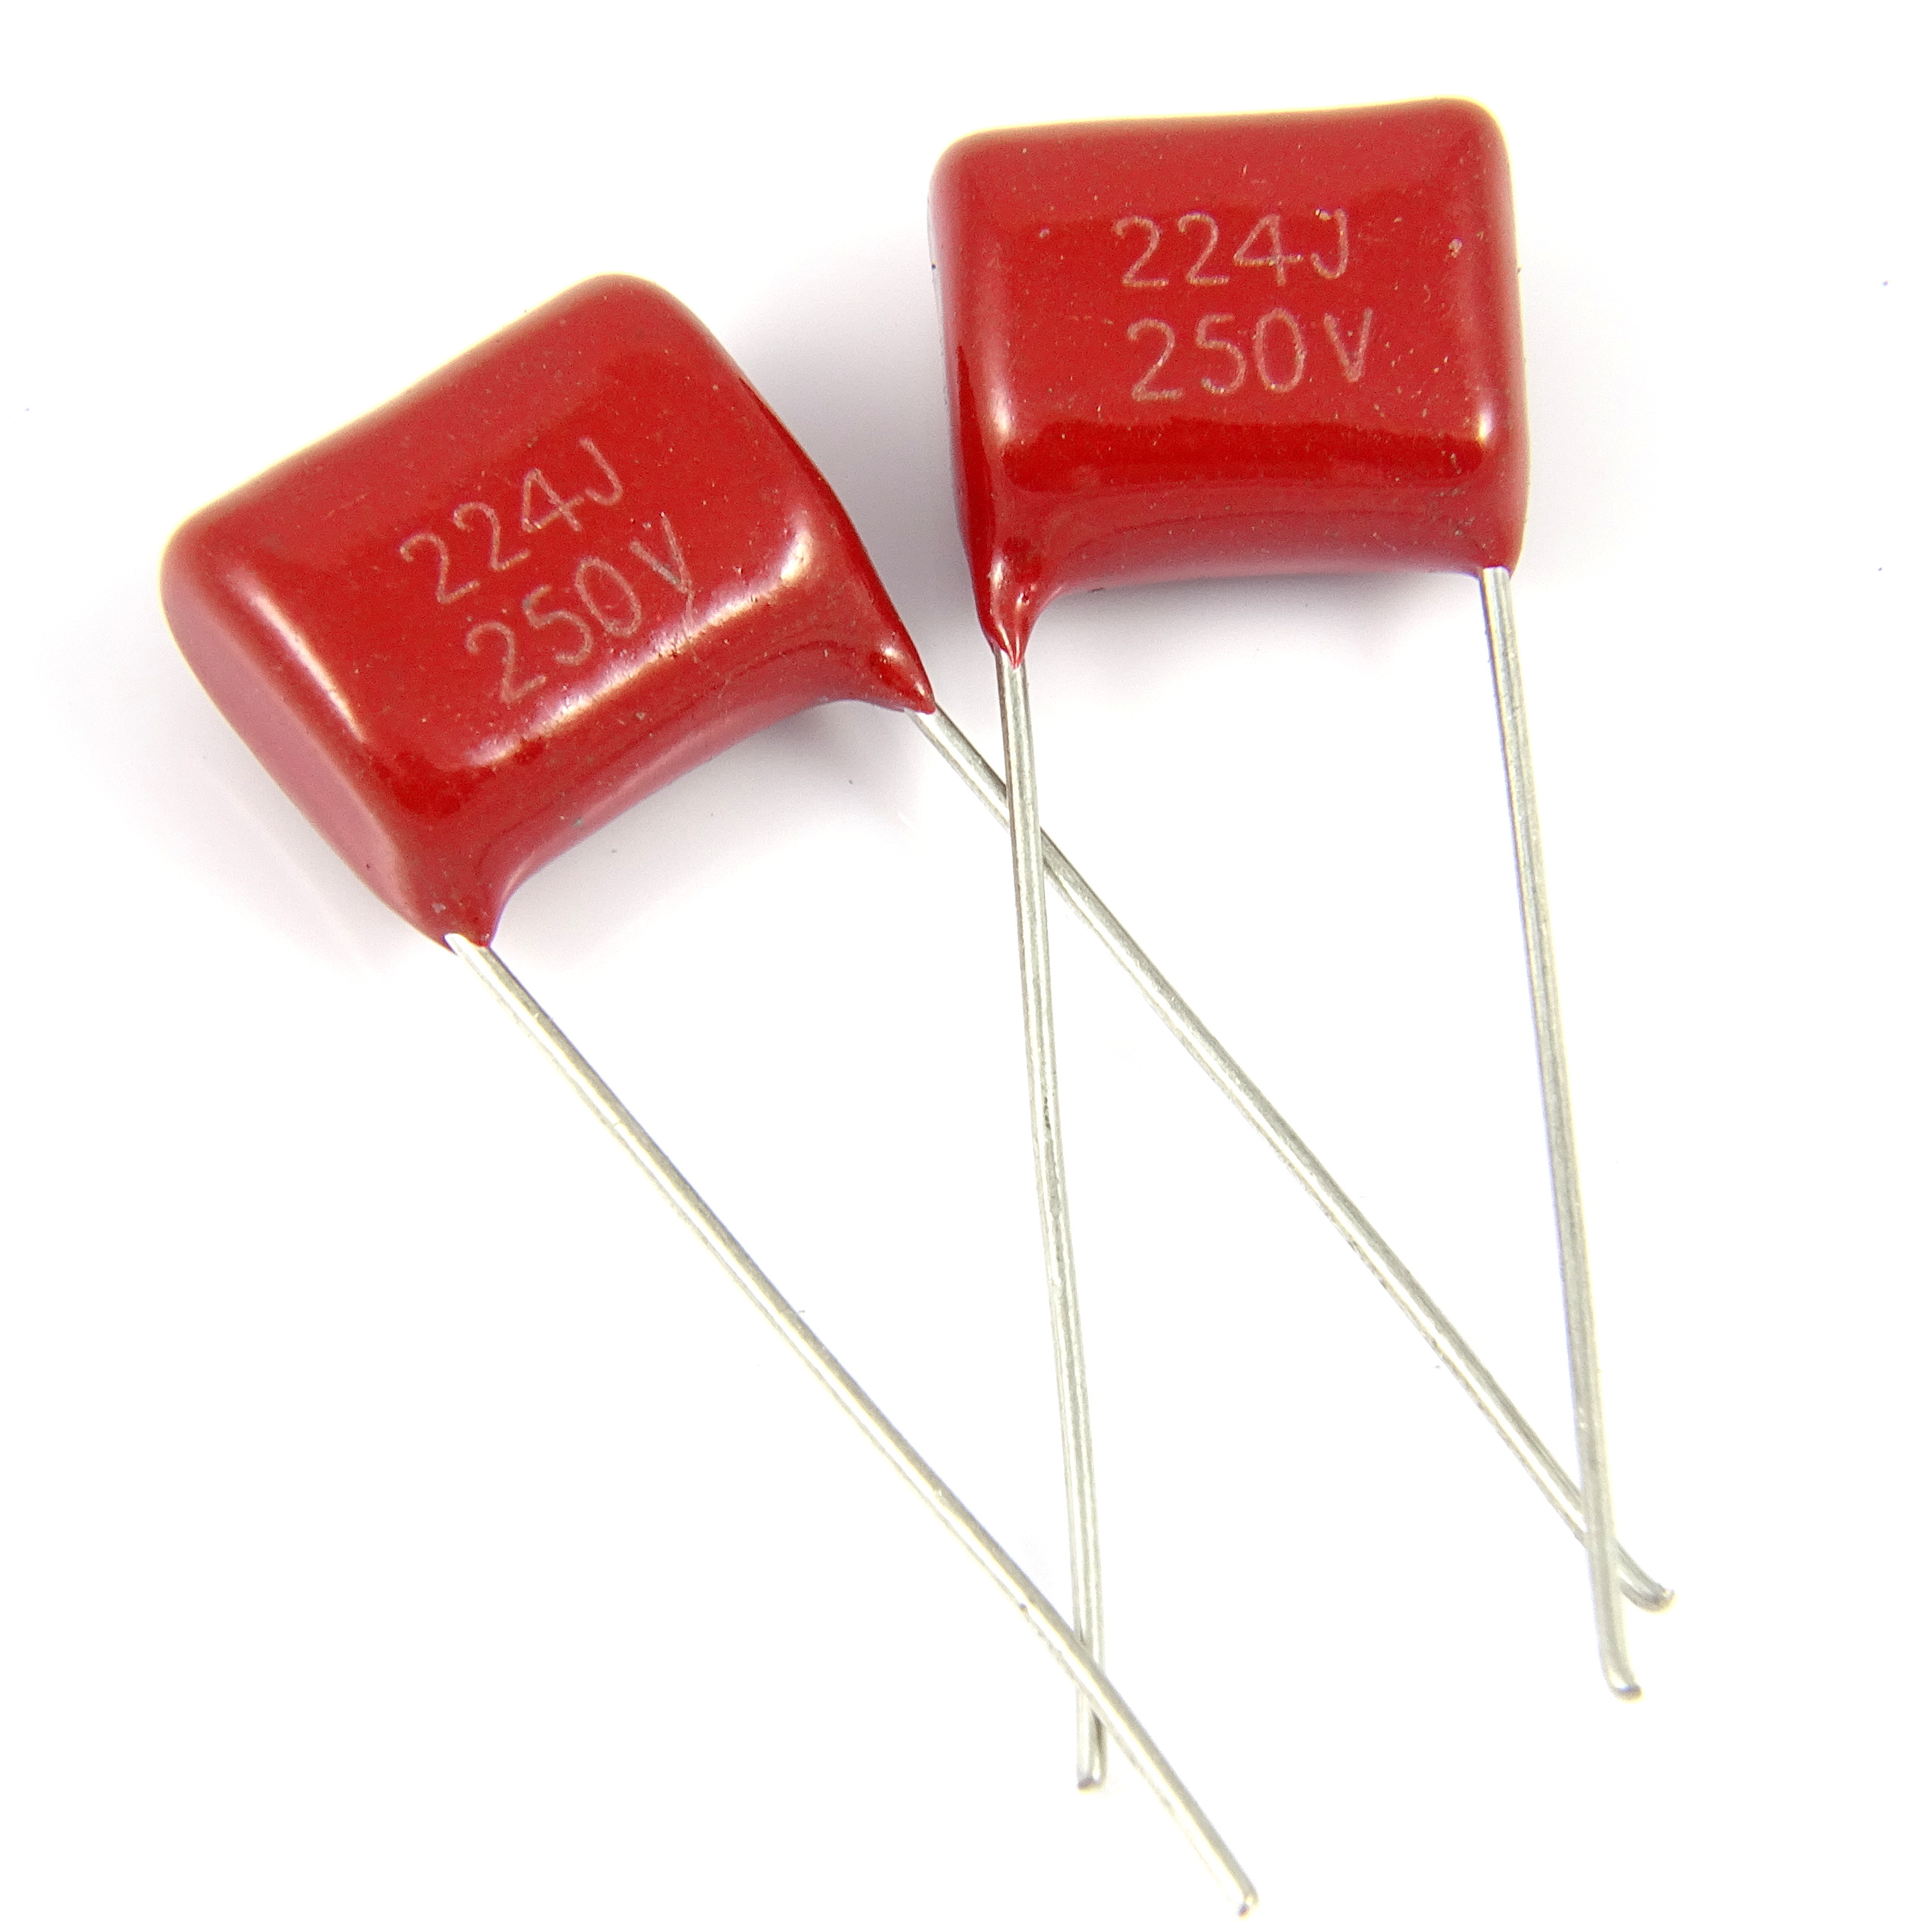
\includegraphics[width=0.50\textwidth]{figures/konding2.jpg}
    }\\
  \end{columns}
\end{frame}

\handoutnoteslide

\mode<beamer>{
%%--------------------------------------------------
%% Ny frame
%%--------------------------------------------------
\begin{frame}{Kondensatorer i kretsar}
  \huge
  \url{https://youtu.be/Oq1JGoG2OQQ}
\end{frame}
} % end mode

%% --------------------------------------------------
%% Ny frame
%%--------------------------------------------------
\begin{frame}[fragile]{Kondensatorer i kretsar}
  \begin{columns}
    \column{0.5\textwidth}
    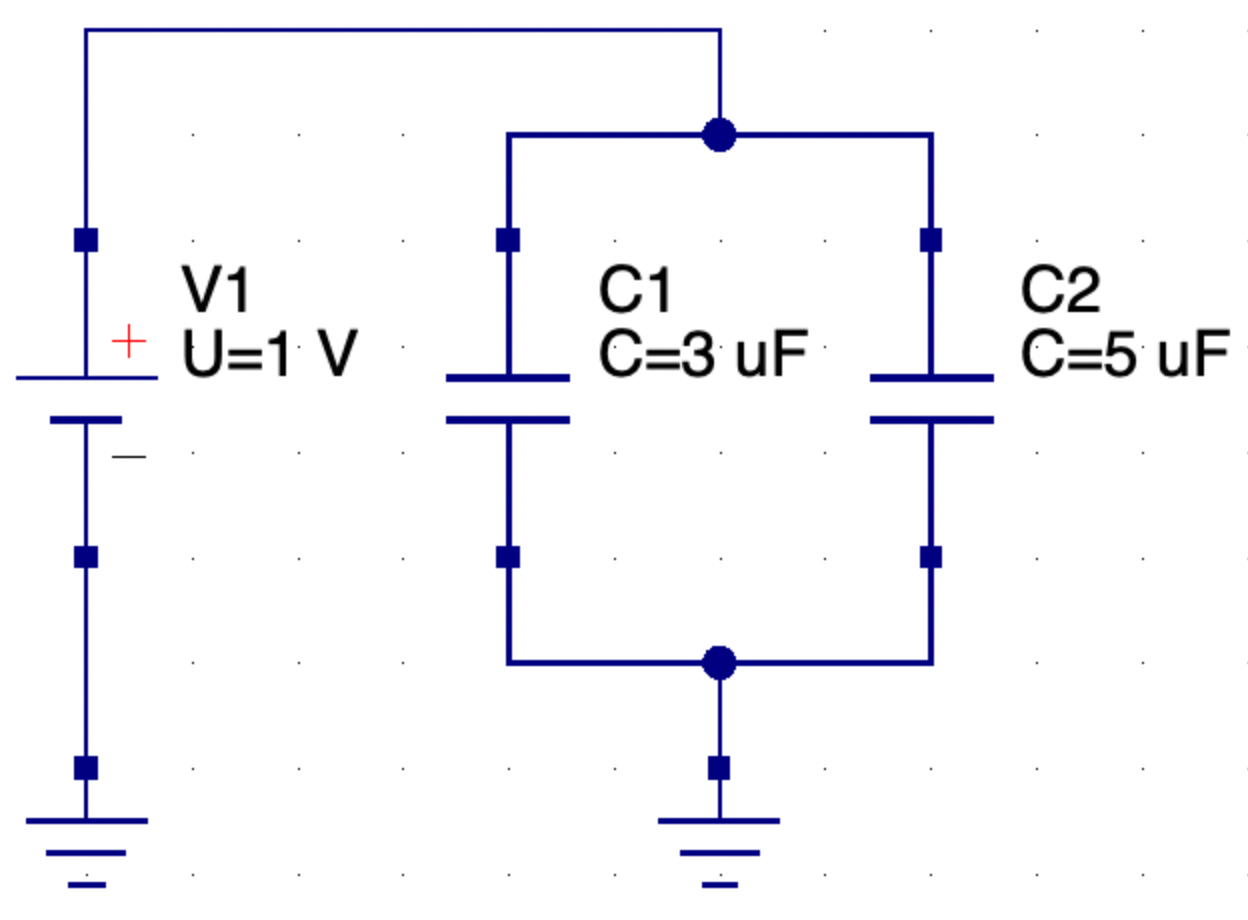
\includegraphics[width=\textwidth]{figures/kondparallell.png}
    \column{0.5\textwidth}
    \begin{itemize}
    \item Bestäm laddningen på kondensatorerna.
    \item Hur stor ström går det i kretsen efter lång tid?
    \end{itemize}
    \onslide<2->{
      $C=\frac{Q}{U}\Rightarrow Q=CU$
    }
  \end{columns}
  \vspace{29mm}
\end{frame}

\handoutnoteslide


% Circuit values: volts, kiloohms and microfarads
\newcommand{\CapSupply}{5}
\newcommand{\CapResistance}{10}
\newcommand{\CapCapacitance}{100}

% Time constant in seconds
\pgfmathsetmacro{\CapTau}{%
    \CapResistance*\CapCapacitance/1000}
\pgfmathsetmacro{\CapEndTime}{5*\CapTau}
\pgfmathsetmacro{\CapPlotMax}{1.1*\CapSupply}

\pgfplotsset{
    capacitor plot/.style={
        width=\linewidth,
        height=0.68\textheight,
        xmin=0,
        xmax=\CapEndTime,
        ymin=0,
        ymax=\CapPlotMax,
        domain=0:\CapEndTime,
        samples=150,
        axis lines=left,
        xlabel={$t$ (s)},
        ylabel={$u_C$ (V)},
        grid=major,
        major grid style={gray!30},
        tick align=outside,
        every axis plot/.append style={very thick, blue!70!black},
    }
}

%------------------------------------------------
\begin{frame}{Charging a capacitor}
    \begin{columns}[c,onlytextwidth]

        \begin{column}{0.43\textwidth}
            \centering
            \begin{circuitikz}[american resistors, scale=0.85]
                \draw
                    (0,0)
                    to[V, l_=$\CapSupply\,\mathrm{V}$] (0,3)
                    to[cute closed switch] (1.5,3)
                    to[R, l=$\CapResistance\,\mathrm{k\Omega}$] (3.5,3)
                    to[C, l_=$\CapCapacitance\,\mu\mathrm{F}$,
                          v^=$u_C$] (3.5,0)
                    -- (0,0);

                \node[above] at (0.75,3.35) {$t=0$};
            \end{circuitikz}

            \medskip
            {\small Switch closes at \(t=0\).\\
            Initially, \(u_C(0)=0\).}

            \medskip
            \[
                \tau=RC=
                \pgfmathprintnumber{\CapTau}\,\mathrm{s}
            \]
        \end{column}

        \begin{column}{0.55\textwidth}
            \centering
            \begin{tikzpicture}
                \begin{axis}[capacitor plot]
                    \addplot {
                        \CapSupply*(1-exp(-x/\CapTau))
                    };
                \end{axis}
            \end{tikzpicture}

            \[
                u_C(t)=U_0\left(1-e^{-t/(RC)}\right)
            \]
        \end{column}

    \end{columns}
\end{frame}

%------------------------------------------------
\begin{frame}{Discharging a capacitor}
    \begin{columns}[c,onlytextwidth]

        \begin{column}{0.43\textwidth}
            \centering
            \begin{circuitikz}[american resistors, scale=0.85]
                \draw
                    (0,0) -- (0,3)
                    to[cute closed switch] (1.5,3)
                    to[R, l=$\CapResistance\,\mathrm{k\Omega}$] (3.5,3)
                    to[C, l_=$\CapCapacitance\,\mu\mathrm{F}$,
                          v^=$u_C$] (3.5,0)
                    -- (0,0);

                \node[above] at (0.75,3.35) {$t=0$};
            \end{circuitikz}

            \medskip
            {\small Switch closes at \(t=0\).\\
            Initially, \(u_C(0)=\CapSupply\,\mathrm{V}\).}

            \medskip
            \[
                \tau=RC=
                \pgfmathprintnumber{\CapTau}\,\mathrm{s}
            \]
        \end{column}

        \begin{column}{0.55\textwidth}
            \centering
            \begin{tikzpicture}
                \begin{axis}[capacitor plot]
                    \addplot {
                        \CapSupply*exp(-x/\CapTau)
                    };
                \end{axis}
            \end{tikzpicture}

            \[
                u_C(t)=U_0 e^{-t/(RC)}
            \]
        \end{column}

    \end{columns}
\end{frame}


%%--------------------------------------------------
%% Ny frame
%%--------------------------------------------------
\begin{frame}[fragile]{Upp- och urladdning av kondensator}
\begin{columns}
         \column{0.4\textwidth}
         \alert{OBS!} Alltid kondensatorer i serie med resistor
         \onslide<2->{
         Spänning i kretsen beskrivs
         av:\[\frac{\mathrm{d}u}{\mathrm{d}t}+\frac{1}{RC}u=0.\]
         \\}
       \onslide<3->{
       \alert{kretsens tidskonstant:} 
           {\huge \[ \tau=RC \] }, \\
         }
         \onslide<4->{
      Efter tiden $\tau$ \alert{63\% av ändringen.}
    }
         \column{0.6\textwidth}
    %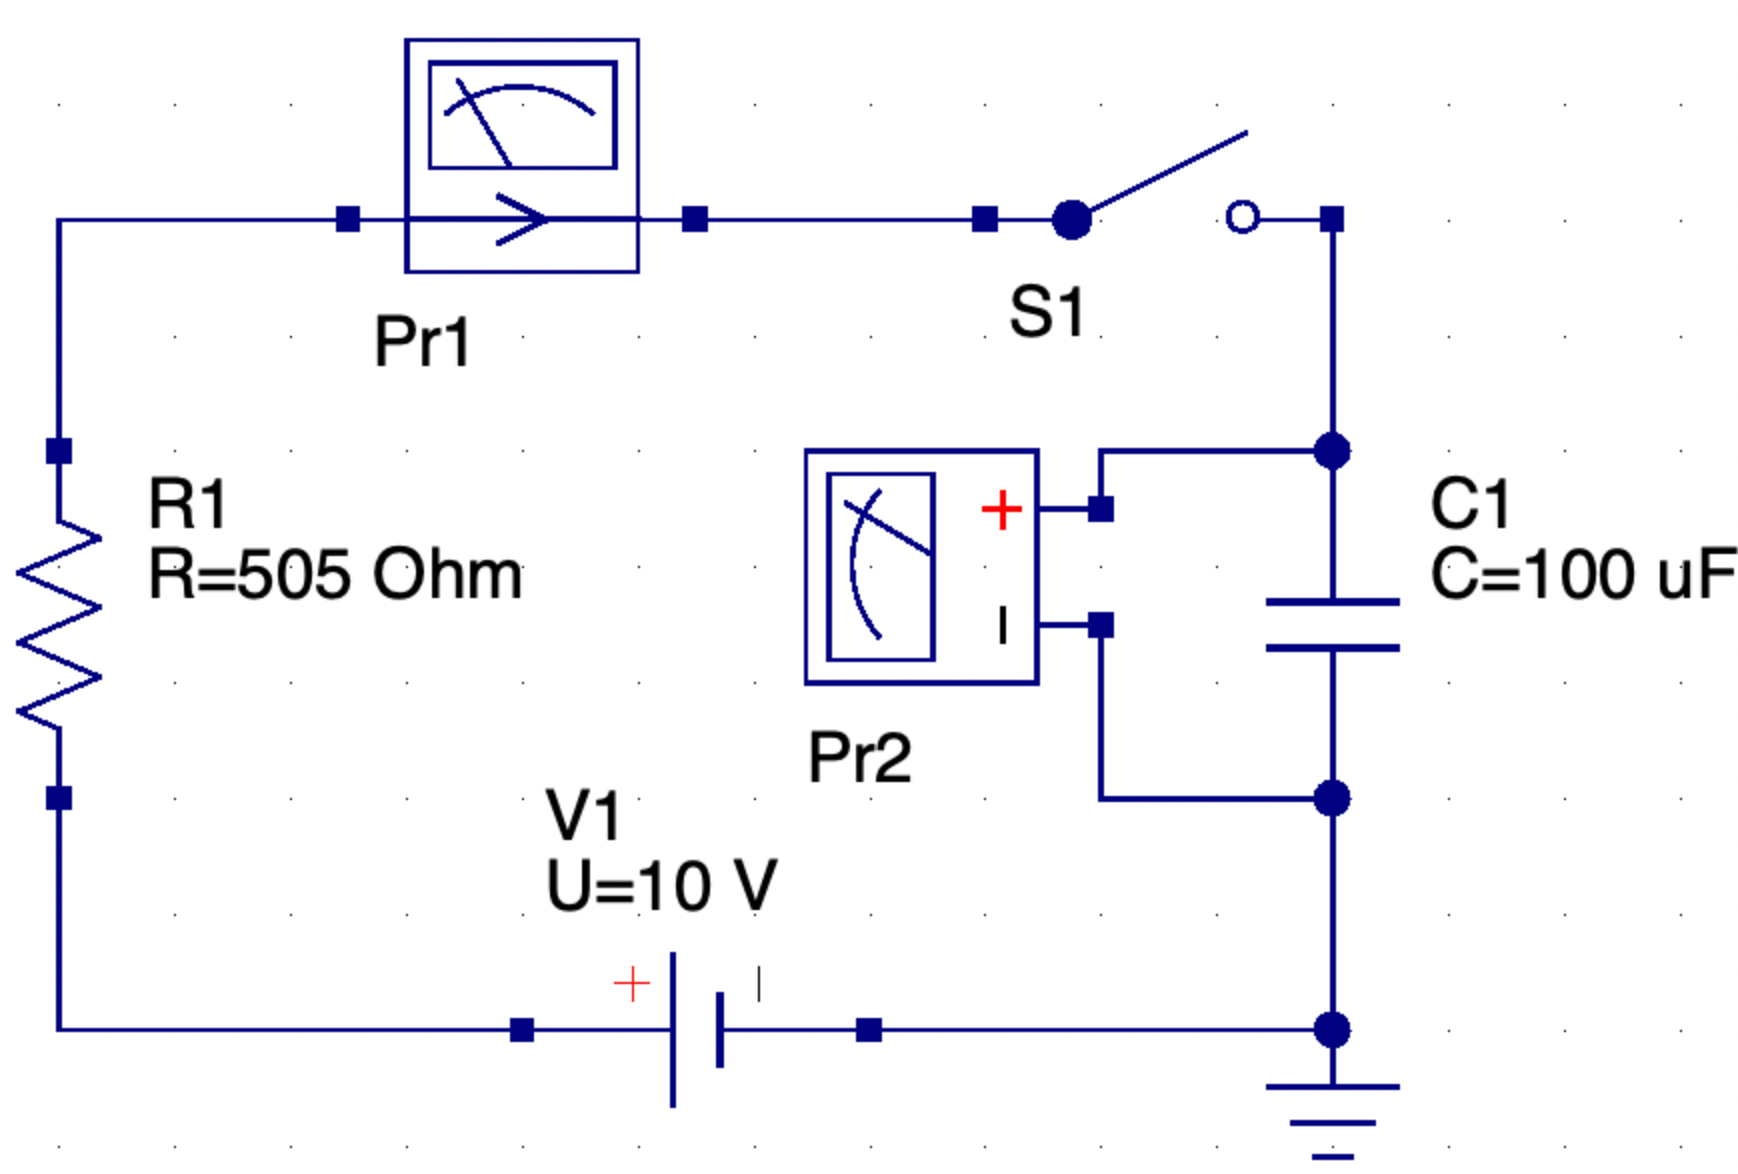
\includegraphics[width=0.75\textwidth]{figures/uppladdning.png}\\
        \centering
         \resizebox{0.5\textwidth}{!}{       
    \begin{circuitikz}[american resistors, scale=0.85]
                \draw
                    (0,0)
                    to[V, l_=$\CapSupply\,\mathrm{V}$] (0,3)
                    to[cute closed switch] (1.5,3)
                    to[R, l=$\CapResistance\,\mathrm{k\Omega}$] (3.5,3)
                    to[C, l_=$\CapCapacitance\,\mu\mathrm{F}$,
                          v^=$u_C$] (3.5,0)
                    -- (0,0);

                \node[above] at (0.75,3.35) {$t=0$};
            \end{circuitikz}}% resizebox
            \\
            \vspace{5mm}
         %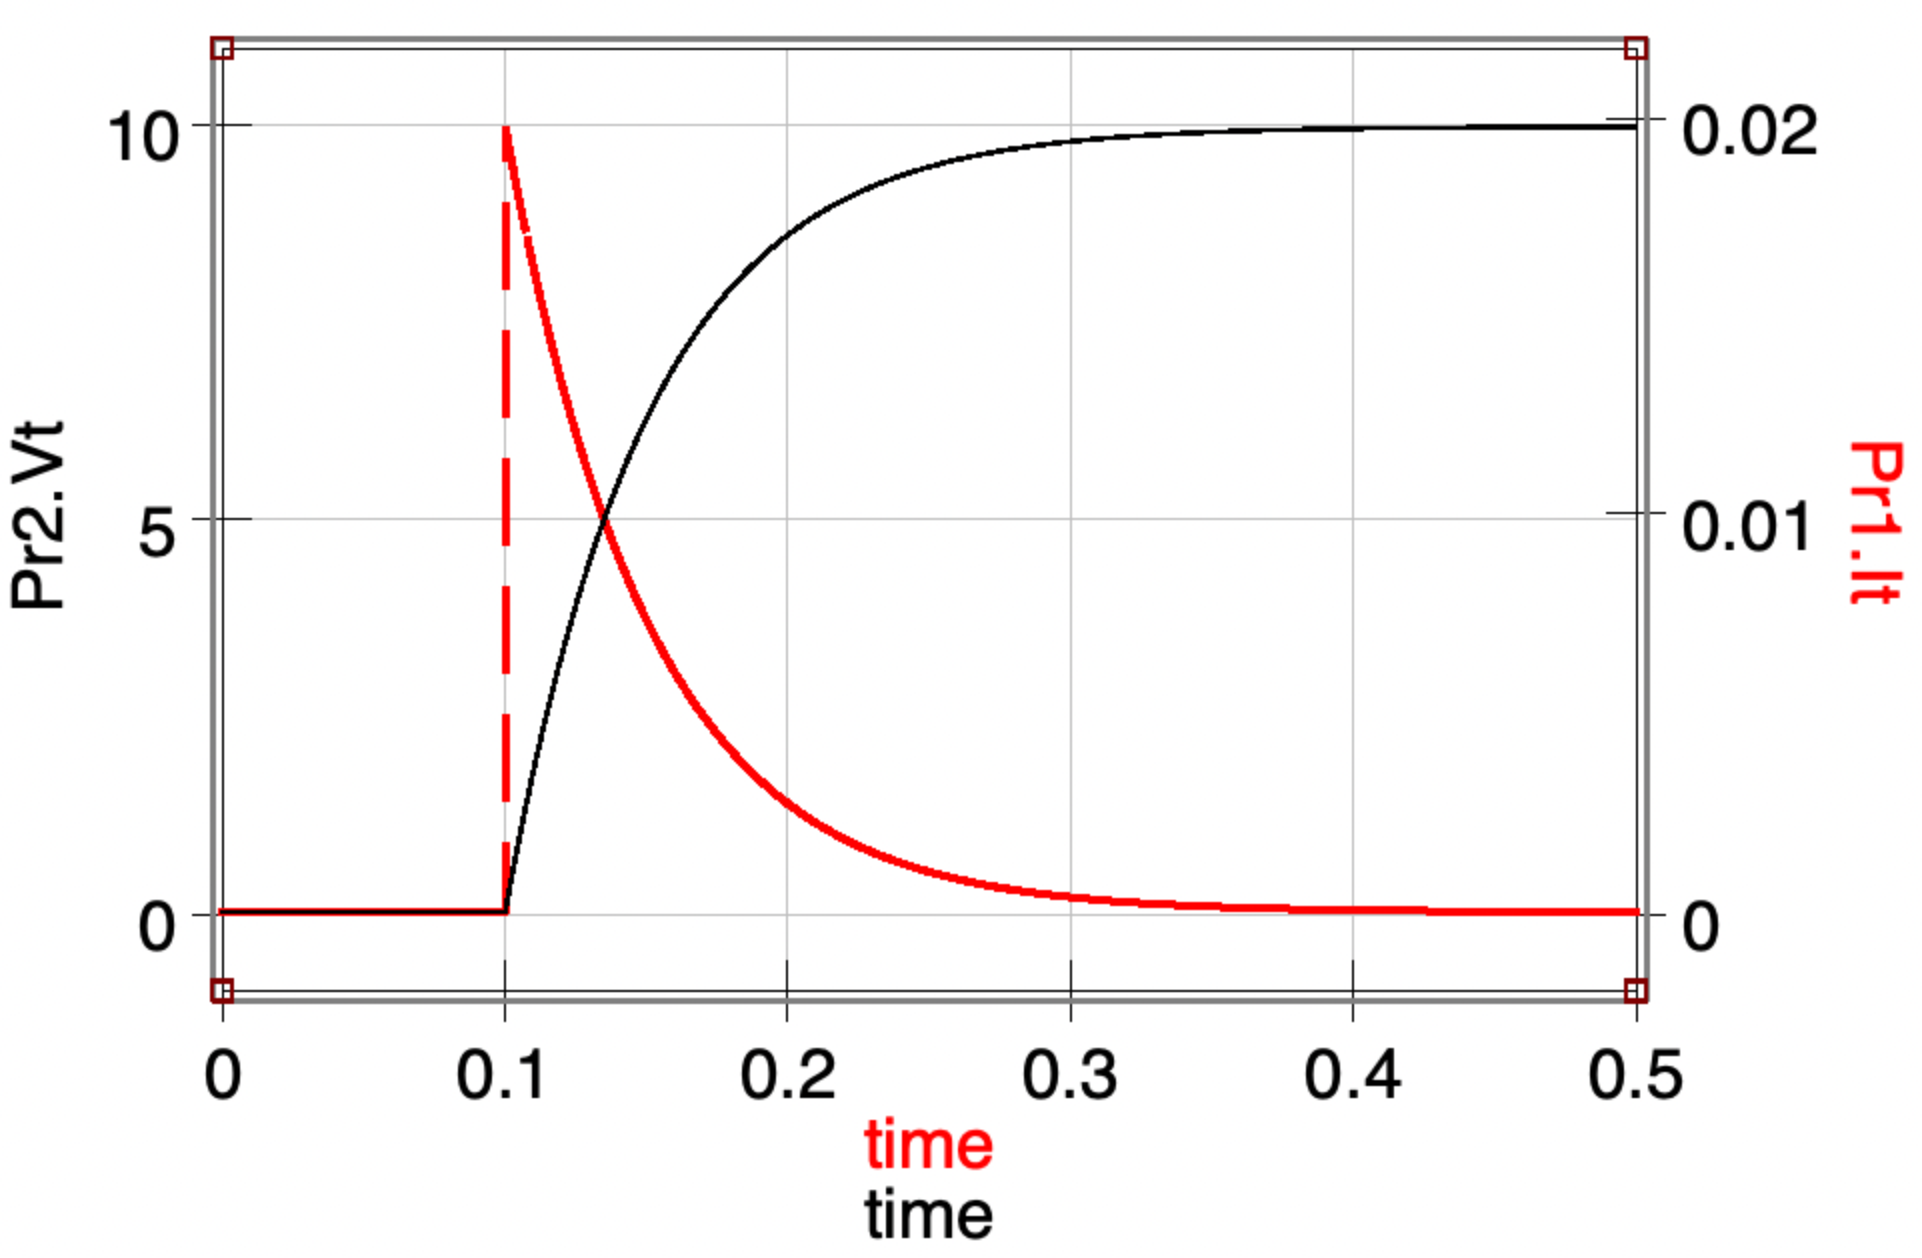
\includegraphics[width=0.75\textwidth]{figures/uppladdning2.png}
         \resizebox{0.7\textwidth}{!}{       
            \begin{tikzpicture}
                \begin{axis}[capacitor plot]
                    \addplot {
                        \CapSupply*(1-exp(-x/\CapTau))
                    };
                \end{axis}
            \end{tikzpicture}
         } % resizebox 

       \end{columns}
\end{frame}

\handoutnoteslide

\frame{
\frametitle{Urladdning av kondensator -- uppkoppling}
\resizebox{0.75\textwidth}{!}{%
\begin{minipage}{.5\textwidth}
\centering
  \begin{circuitikz}[american] \draw
    (0, 0)  to[american voltage source, invert, v=$U$] (0,2)
    (0, 2) to[opening switch] (2, 2)
    to[eC=$C$, *-*] (2,0)
    (2,2) -- (4, 2)
    to[R=$R$, *-*] (4, 0)
	(0, 0)
    node[ground]{}
    (0, 0) -- (4, 0)
    (4, 2) to[short, -*] (6, 2)
    (4, 0) to[short, -*] (6, 0)
    (6,2) to [open, v^>=$U_{ut}$] (6,0) 
    ;
  \end{circuitikz}
\end{minipage}
}\\\vspace{3mm}
{\Large $U<U_\text{max}$. $\tau = RC \approx \qty{1}{\min}$.\\\vspace{1mm} Nedteckna $U_{ut}$ minst 15 ggr tills $t > 1.5\tau$. \\\vspace{1mm}
Presentera \alert{tydliga} grafer!}
}

\handoutnoteslide

\mode<beamer>{
%%--------------
%% Ny frame
%%--------------
\begin{frame}{Urladdning av kondensator -- resultat}
  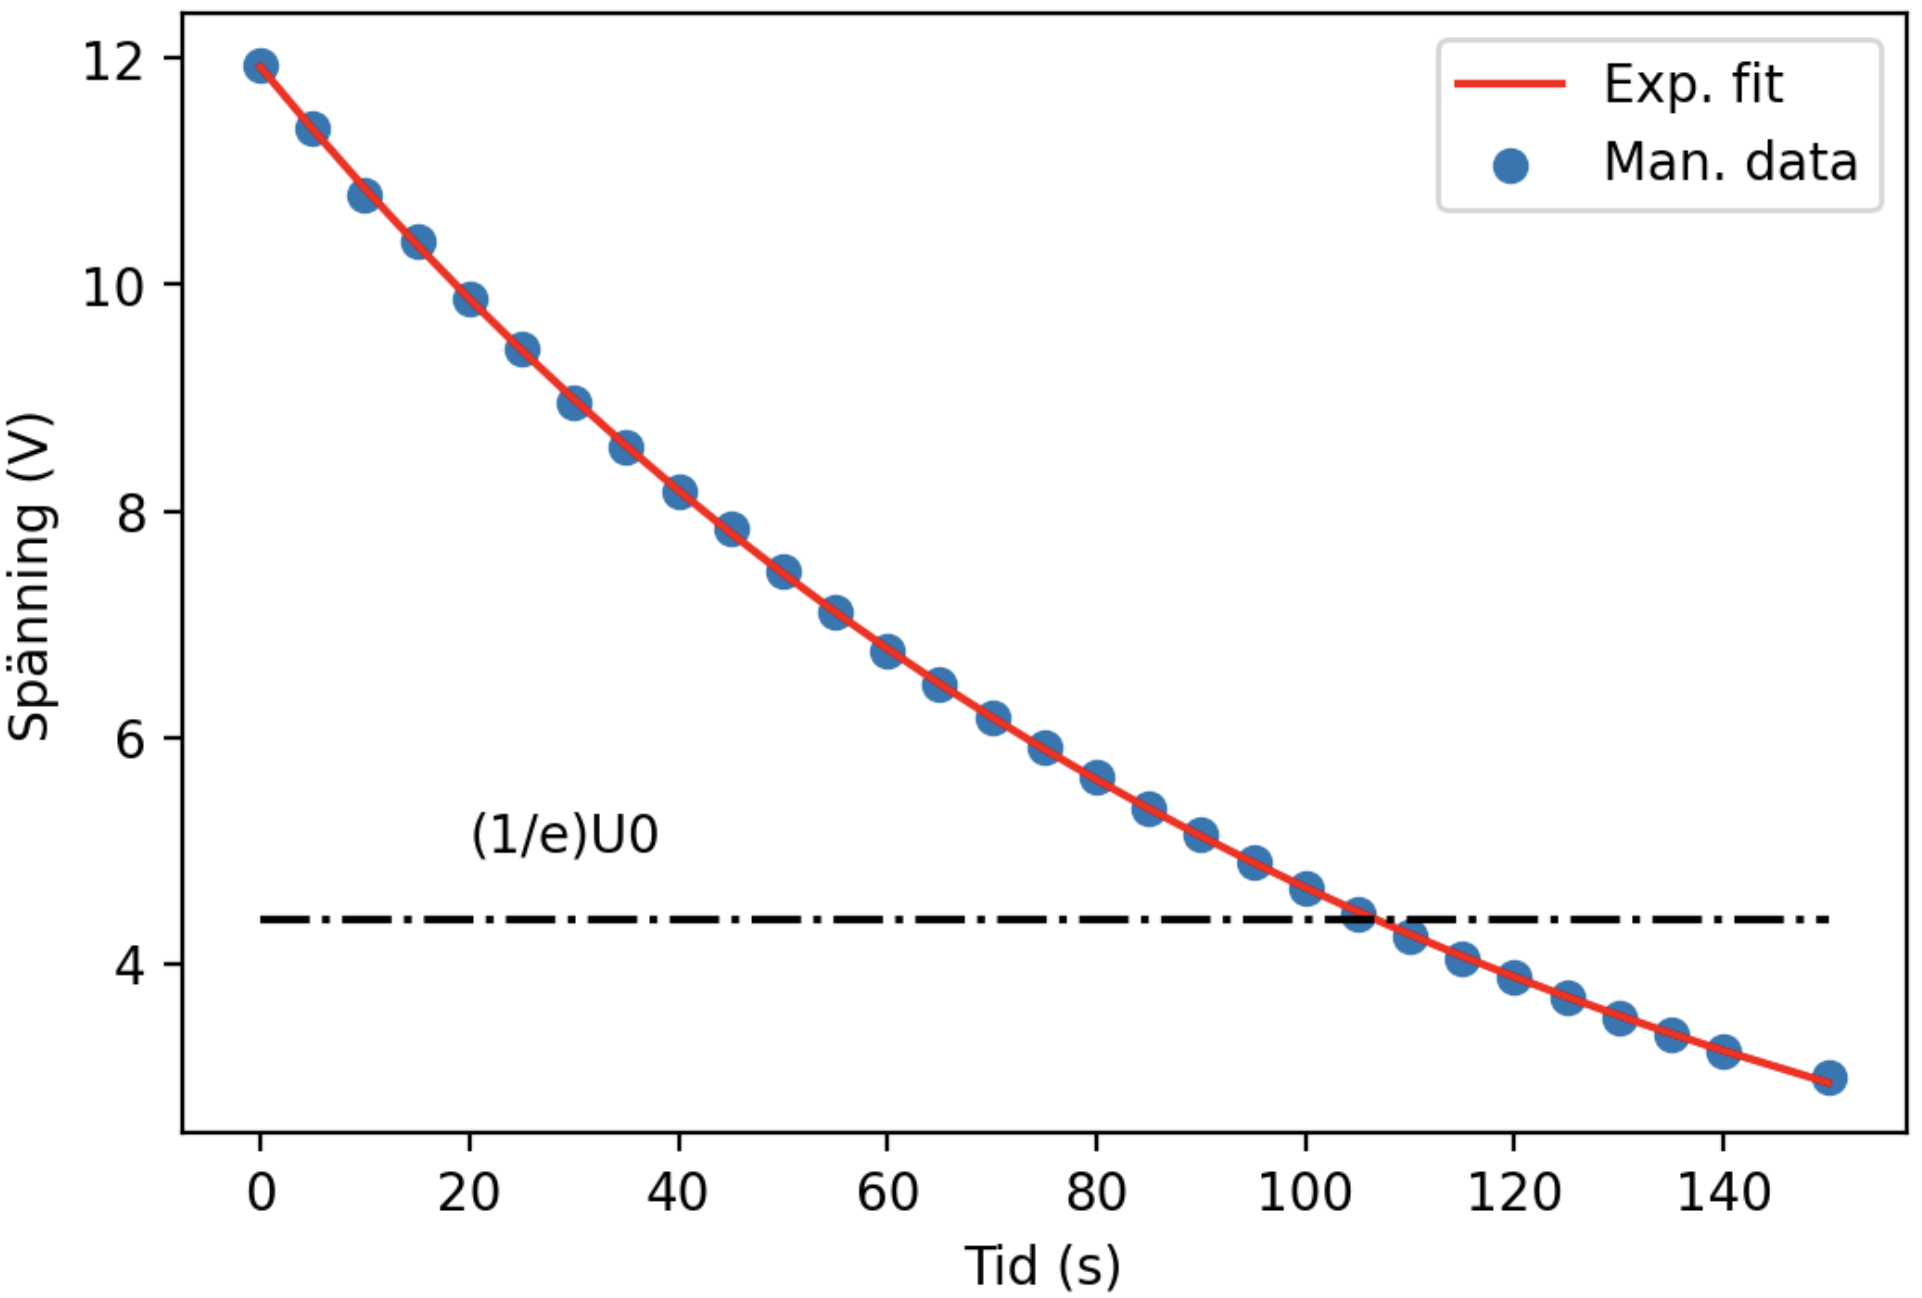
\includegraphics[width=0.9\textwidth]{figures/konding_labb.png}
\end{frame}
}%end mode

\mode<handout>{
\begin{frame}[plain]
    \centering
    \begin{tikzpicture}
        \begin{axis}[
            width=0.97\paperwidth,
            height=0.94\paperheight,
            anchor=center,
            scale only axis=false,
            xmin=0, xmax=10,
            ymin=0, ymax=6,
            axis lines=left,
            axis line style={->},
            xtick={0,1,...,10},
            ytick={0,1,...,6},
            xticklabels=\empty,
            yticklabels=\empty,
            tick style={draw=none},
            grid=major,
            major grid style={gray!40, thin},
            enlargelimits=false,
        ]
        \end{axis}
    \end{tikzpicture}
\end{frame}
} % end mode

\handoutnoteslide

\mode<beamer>{
\frame{
\frametitle{}
{\Huge Växelström och likström}
}
} % end mode

%% --------------------------------------------------
%% Ny frame
%%--------------------------------------------------

\begin{frame}[fragile]{\emph{Direct Current} och \emph{Alternating Current}}

\begin{columns}
  \column{0.7\textwidth}
  DC -- Likström

  \column{0.3\textwidth}<3->
  AC -- Växelström
  \end{columns}
\vspace{2mm}
  \begin{columns}
  \column{0.33\textwidth}
  \begin{circuitikz}[american] \draw
    node[ground]{}
    (2, 0)  to[V=\SI{1}{\volt}] (0,0)
    (2, 0) to[short, -, i=$I_0$] (2, 2)
    (2, 2) to[R=\SI{50}{\ohm}] (0,2)
    (0, 2) to[short, -*, i=$I_0$] (0, 0)
  ;
\end{circuitikz}

\column{0.33\textwidth}<1->
  \begin{circuitikz}[american] \draw
    node[ground]{}
  (2, 0)  to[battery1=\SI{1}{\volt}] (0,0)
    (2, 0) to[short, -, i=$I_0$] (2, 2)
    (2, 2) to[R=\SI{50}{\ohm}] (0,2)
    (0, 2) to[short, -*, i=$I_0$] (0, 0)
  ;
\end{circuitikz}
\column{0.33\textwidth}<3->
  \begin{circuitikz}[american] \draw
    node[ground]{}
 (2,0) to[sinusoidal voltage source, l=\SI{1}{\volt}\,$\sin{\omega t}$] (0,0)
    (2, 0) to[short, -, i=$i_0$] (2, 2)
    (2, 2) to[R=\SI{50}{\ohm}] (0,2)
    (0, 2) to[short, -*, i=$i_0$] (0, 0)
 ;
\end{circuitikz}
\end{columns}\vspace{2mm}
\begin{columns}<2->
  \column{0.6\textwidth}
  Ohms lag ger:
  \[I_0=\frac{\SI{1}{\volt}}{\SI{50}{\ohm}}=\SI{20}{\milli\ampere}\]

  \column{0.4\textwidth}<4->
  Ohms lag ger (också):
  \[i_0=\frac{\SI{1}{\volt}\sin{\omega
        t}}{\SI{50}{\ohm}}=\SI{20}{\milli\ampere}\sin\omega t\]
\end{columns}
\end{frame}

\handoutnoteslide


%%--------------------------------------------------
%% Ny frame
%%--------------------------------------------------
\begin{frame}[fragile]{Växelström och växelspänning}
%\begin{columns}
%\column{0.2\textwidth}
%	
%	\begin{itemize}
%		\item<2-> Amplitud\\$u$-hatt, $\hat{u}$ \\$i$-hatt, $\hat{i}$
%		\item<3-> Frekvens\\Periodtid
%	\end{itemize}
%	\onslide<4->{
%	Effektivvärde\\samma \alert{effekt} som DC\\
%	$I_\text{eff}=\frac{\hat{i}}{\sqrt{2}}$
%	}
%\column{0.8\textwidth}
	\begin{tikzpicture}[scale=1.5]
	\datavisualization [scientific axes, visualize as smooth line,
						x axis={label=Tid (\unit{\micro\s}), ticks={
						major={at={0,90,180,270,360}}}},y axis={
						label=Spänning (\unit{\mV}), ticks={
						major={at={-1, -0.75,-0.5,-0.25,0,0.25,0.5,0.75,1}}}}]
		data [format=function] {
			var x : interval [-5:365];
			func y = sin( \value x );
			};
		\onslide<2->{
		% amplitudoverlay
		\draw (1.5,2.32) node[anchor = west, red] 
		{Amplitud, $\hat{u}=\qty{1}{\mV}$} ;
		\draw[red, very thick, |-|] (1.285,1.55) -- (1.285, 3.09) ;	
		}
		\onslide<3->{
		% Periodtidoverlay
		\draw (2.5,1.5) node[anchor = north, blue] {Periodtid, 
		$T=\frac{1}{f}=\qty{360}{\us}\Rightarrow f\approx\qty{2.78}{\kHz}$} ;
		\draw (0.7, 1.0) node[anchor = west, blue] {Vinkelfrekvens, $\omega = 2 \pi f\approx\qty{17.4}{\kilo\radian\per\s}$} ;
		\draw[blue, very thick, |-|] (0.06,1.545) -- (4.94, 1.545) ;
		}
	\end{tikzpicture}\\
	\onslide<4->{
	\[ u(t) = \qty{1}{\mV} \sin \big( \qty{17.4}{\kilo\radian\per\s} t \big) \]
	}
%\end{columns}
\end{frame}


\handoutnoteslide


%%--------------------------------------------------
%% Ny frame
%%--------------------------------------------------
\begin{frame}[fragile]{Växelström - Resistorn}
	\begin{columns}
		\column{0.3\textwidth}
			\alert{Växelspänning}
			$$u(t) = \hat{u}\sin\omega{}t$$
			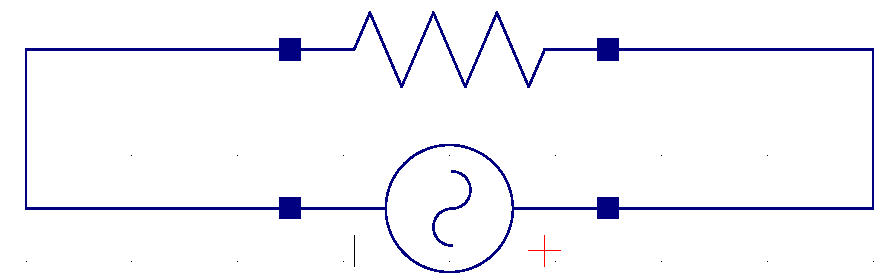
\includegraphics[width=\textwidth]{figures/URcircuit.png}		\\
				\onslide<3->{\alert{Ohms vanliga lag gäller:} $u=R\cdot{}i$\\ }
        \onslide<3->{både amplituder och effektivvärden.}

		\column{0.7\textwidth}<2->
			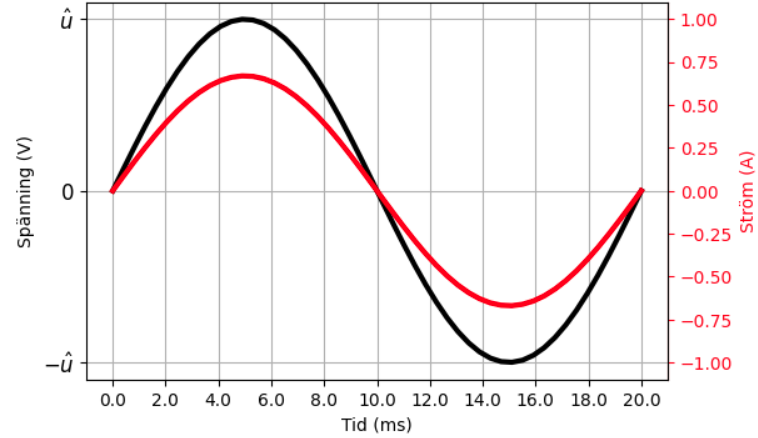
\includegraphics[width=\textwidth]{figures/URI.png}
	\end{columns}
%	\vspace{10mm}
\end{frame}

\handoutnoteslide


%%--------------------------------------------------
%% Ny frame
%%--------------------------------------------------
\begin{frame}[fragile]{Växelström - Kondensatorn}
	\begin{columns}
		\column{0.3\textwidth}
			\alert{Växelspänning}
			$$u(t) = \hat{u}\sin\omega{}t$$
			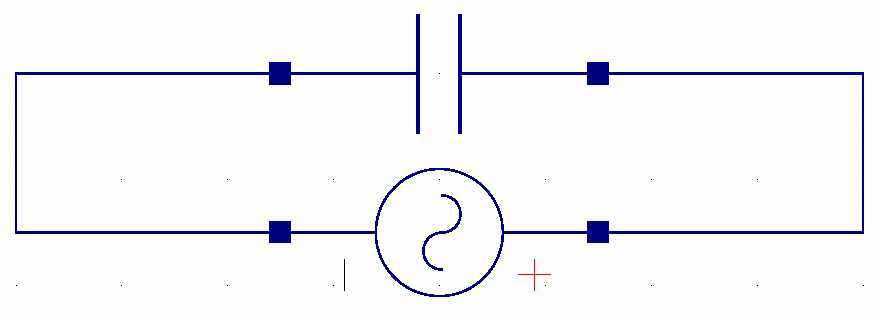
\includegraphics[width=\textwidth]{figures/UCcircuit.png}	\\
			        \onslide<3->{Strömmen går \SI{90}{\degree} \emph{före} spänningen.\\}
        \onslide<4->{Ohms lag $U=\frac{1}{\omega C}I$ effektivvärden och amplituder.}

		\column{0.7\textwidth}<2->
			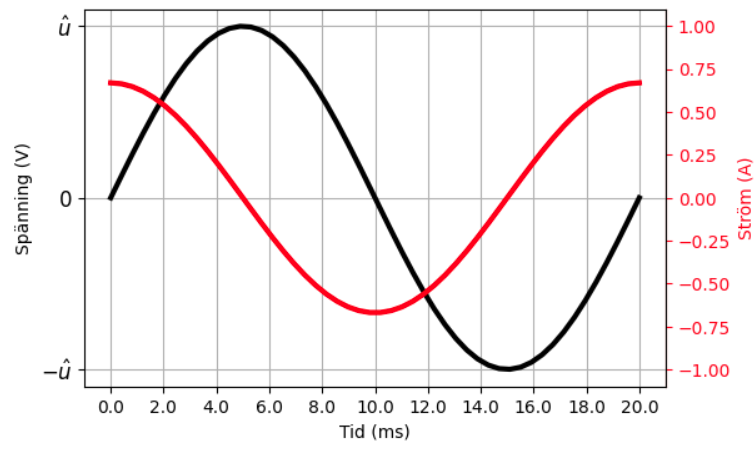
\includegraphics[width=\textwidth]{figures/UCI.png}
	\end{columns}
	\vspace{5mm}
	\begin{center}
	\onslide<5->{
		$\frac{1}{\omega C}$ kapacitiva \alert{reaktansen} $X_C$ (\unit{\ohm})
	}
	\end{center}
\end{frame}

\handoutnoteslide

%%--------------------------------------------------
%% Ny frame
%%--------------------------------------------------
\begin{frame}[fragile]{Växelström - Kondensatorn}
	
	{\LARGE
	Över en kondensator med kapacitansen \qty{0.1}{\uF} ligger spänningen 
	$u(t) = \qty{100}{\V}\sin 400 \pi t$. Beräkna amplituden hos strömmen genom
	kondensatorn.
	}
	\vspace{40mm}
	\mode<beamer>{
  \onslide<2->{
	\[U=\frac{1}{\omega C}I \Rightarrow \hat{i} = \hat{u}\omega C = \qty{100}{\V}
	\pi\qty{400}{\radian\per\s}\qty{0.1}{\uF}\approx\qty{12.6}{\mA}\]
	}
  } % end mode
\end{frame}

\handoutnoteslide


\end{document}
